\section{Ранг матрицы}

\begin{definition}
   Набор матриц назовем \textit{линейно зависимым}, если существует нетривиальная линейная комбинация, равная нулевой матрице. 
\end{definition}

Все теоремы о линейной зависимости для векторов верны и для матриц.\\

\begin{theorem}
    Если некоторая матрица раскладывается на линейную комбинацию некоторого набора матриц, то это разложение единственно тогда и только тогда, когда этот набор линейно независимый.
\end{theorem}
\begin{proof}
    \tab\\
    
    Доказательство аналогично доказательству соответствующей теоремы для векторов.
\end{proof}

Пусть набор строк произвольной матрицы А линейно зависим, т.е. существует ненулевая строка $\overline{c}$ такая, что \textbf{$\overline{c}A = \overline{0}$}.

\begin{theorem}
    Пусть А, В $-$ квадратные матрицы, а строки А линейно зависимы. Тогда строки АВ тоже инейно зависимы.
\end{theorem}
\begin{proof}
    \tab\\
    
    Строки А - линейно зависимые $\Longleftrightarrow$ $\exists \overline{c}\neq\overline{0} : \overline{c}A = \overline{0}$. Тогда
    \[
    \overline{c}(AB) = (\overline{c}A)B = \overline{0} \cdot B = \overline{0}
    \]
    Значит, набор строк АВ линейно зависим.
\end{proof}

\begin{theorem}
    Элементарные преобразования строк (столбцов) переводят линейно независимый набор в линейно независимый, а линейно зависимый в линейно зависимый.
\end{theorem}
\begin{proof}
    \tab\\
    \begin{enumerate}
        \item Пусть $\overline{a_1}, ..., \overline{a_k}$ $-$ линейно независимый набор.\\
        Пусть к первой строке прибавили вторую: $\overline{a_1} + \overline{a_2}, \overline{a_2}, ..., \overline{a_k}$. Тогда линейная комбинация: $\alpha_1(\overline{a_1} + \overline{a_2}) +  \alpha_2\overline{a_2} + ... + \alpha_k\overline{a_k}$ или $\alpha_1\overline{a_1}  +  (\alpha_1 + \alpha_2)\overline{a_2} + ... + \alpha_k\overline{a_k}$ $\Longrightarrow$ т.к. набор линейно независимый, линейная комбинация равна нулю, когда $\alpha_1 = 0$, $\alpha_1 + \alpha_2 = 0$ $\Longrightarrow$ $\alpha_2 = 0$, ..., $\alpha_k = 0$. Получили тривиальный набор коэффициентов, значит новый набор тоже линейно независимый.
        \item Предположим противное и получим противоречие, т.к. элементарные операции обратимы.
    \end{enumerate}
\end{proof}

\begin{theorem}
    При элементарных преобразованиях со столбцами (строками) линейная зависимость строк (столбцов) сохраняется.
\end{theorem}
\begin{proof}
    \tab\\
    Пусть А $-$ матрица с линейно зависимыми строками. Тогда $\exists \overline{c}\neq\overline{0} : \overline{c}A = \overline{0}$. Пусть мы провели некоторые элементарные операции с А, т.е. получили элементарную матрицу S. Тогда
    \[
    \overline{c}(AS) = (\overline{c}A)S = \overline{0}
    \]
\end{proof}

\begin{theorem}
    det A = 0 $\Longleftrightarrow$ строки (столбцы) А линейно зависимы.
\end{theorem}
\begin{proof}
    \tab\\
    $\Longleftarrow$\\
    Какая-то строка $-$ линейная комбинация остальных $\Longrightarrow$ элементарные преобразования $\Longrightarrow$ det A = 0\\

    $\Longrightarrow$\\
    Пусть det A $\neq$ 0, тогда через элементарные преобразования строк А можно привести к единичной матрице, но ее строки линейно независимые, пришли к противоречию.
\end{proof}

\begin{theorem}
    Пусть квадратная матрица А не вырождена. Тогда для любого столбца (строки) $\overline{d}$ высоты n существует и единственнен набор коэффициентов $\overline{x} = x_1, ..., x_n$ : $A\overline{x} = \overline{d}$
\end{theorem}

Далее будем говорить о матрицах произвольного размера, если не обговорено обратное.

\begin{definition}
    Пусть имеется матрица А, у которой существует линейно независимый набор из $r_1$ строк, а $\forall r > r_1$ набор линейно зависим или не существует. Тогда будем говорить, что $r_1 = r_1(A)$ $-$ \textit{строчный ранг матрицы А}.\\

    \textit{Строчный ранг матрицы А} $-$ максимальное количество строк, принадлежащих матрице А и образующих линейно независимый набор.
    
\end{definition}

Любой линейно независимый набор из $r_1(A)$ строк матрицы А будем называть \textit{базисом}, а строки \textit{базисными}.

\begin{theorem}
    Любая строка матрицы равна линейной комбинации базисных.
\end{theorem}
\begin{proof}
    \tab\\
    \begin{enumerate}
        \item Эта строка базисная, значит просто обнуляем все строки в комбинации, кроме нее.
        \item Эта строка, обозначим как $\widetilde{a}$, не является базисной. Пусть $a_1, ..., a_m$ $-$ базисные, тогда $a_1, ..., a_m, \widetilde{a}$ $-$ линейно зависимый набор, по определению строчного ранга $\Longrightarrow$ существует нетривиальная комбинация равная нулю, т.е. 
        \[
        \alpha_1a_1 + ... + \alpha_ma_m + \beta\widetilde{a} = 0
        \]
        При этом $\beta\neq0$, т.к. в противном случае это был бы линейно независимый набор $\Longrightarrow$ $\widetilde{a}$ можно выразить через базисные строки.
    \end{enumerate}
\end{proof}

\begin{definition}
    Аналогично строчному рангу определяется столбцовый ранг $r_2(A)$ $-$ максимальное количество столбцов, принадлежащих матрице А и образующих линейно независимый набор.
\end{definition}

\begin{note}
    Базисные строки (столбцы) не всегда определяются единственным образом.
\end{note}

\begin{proposition}
    Элементарные операции со строками и столбцами не меняют строчный и столбцовый ранги.
\end{proposition}

\begin{proposition}
    Пусть $A'$ $-$ подматрица А. Тогда
    \[
    r_1(A') \leq r_1(A)
    \]
    \[
    r_2(A') \leq r_2(A)
    \]
\end{proposition}
\begin{proof}
    \tab\\
    
    Если в А некоторый набор строк (столбцов) линейно зависим, то в A' набор строк (столбцов), которые являются частями изначальных также линейно зависим с теми же коэффициентами.
\end{proof}

\begin{theorem}
    Пусть имеется набор, состоящий из n + 1 столбца (строки) высоты n. Тогда этот набор всегда будет линейно зависимым.
\end{theorem}
\begin{proof}
    \tab\\

    Пусть заданы столбцы $a_1, ..., a_{n + 1}$.\\

    Для $a_1, ..., a_n$ возможны 2 случая:
    \begin{enumerate}
        \item Этот поднабор линейно зависим, тогда весь набор линейно зависим.
        \item Этот поднабор линейно независим, тогда $\exists x = x_1, ..., x_n : Ax = a_{n + 1}\thinspace (det\thinspace A \neq 0)\thinspace \Longrightarrow$ набор линейно зависим.
    \end{enumerate}
\end{proof}

\begin{theorem}
    У любой матрицы А $r_1(A) = r_2(A)$.
\end{theorem}
\begin{proof}
    \tab\\

    Будем рассматривать ненулевую матрицу, т.к. для нулевой тривиально.\\

    С помощью элементарных операций обнулим небазисные строки и получим матрицу $A'$ с $r_1(A)$ ненулевых строк. Линейная зависимость при элементарных операциях сохраняется, значит базисные столбцы остались теми же, что и в А.\\

    Рассмотрим D $-$ матрицу, состоящую из пересечения базисных строк и столбцов $A'$ $\Longrightarrow$ $r_1(A) \geq r_2(A)$, т.к. $r_1$ $-$ высота столбцов D, а $r_2$ $-$ их количество.\\

    Транспонируем матрицу А и аналогичным способом получим $r_1(A) \leq r_2(A)$\\

    Итого $r_1(A) = r_2(A)$
\end{proof}

\begin{proposition}
    Пусть $B_{k\times k}$ $-$ невырожденная подматрица А. Тогда строки (столбцы) А, содержащие В являются линейно независимыми.
\end{proposition}
\begin{proof}
    \tab\\

    Если бы строки (столбцы) А были линейно зависимыми, то и их части, являющиеся строками (столбцами) В, были бы линейно зависимыми. Но тогда B $-$ вырожденная матрица, получили противоречие.
\end{proof}

\begin{corollary}
    Не существует невырожденной подматрицы А размера $k\times k$ такой, что
    \[
    k < rg\thinspace A
    \]
\end{corollary}

Таким образом, доказана \textbf{теорема о ранге матрицы}:
\[
\forall A \hookrightarrow r_1(A) = r_2(A) = r,
\]
где r - максимальный размер невырожденной подматрицы A. Эта подматрица является базисной.

\begin{definition}
    \textit{Минорный ранг} $-$ максимальный размер невырожденной подматрицы.
\end{definition}








\begin{theorem}[О базисном миноре]
    Любая строка (столбец) матрицы может быть представлена как линейная комбинация строк (столбцов), содержащих базисный минор.
\end{theorem}
\begin{proof}
    \tab\\

        Достаточно доказать, что строки (столбцы), содержащие базисный минор линейно независимые.\\

        Предположим противное: если они линейно зависимы, то базисный минор $-$ вырожденная матрица, что противоречит определению.\\

        А т.к. строки (столбцы) линейно независимы и их количество равно рангу матрицы, они являются базисными.
\end{proof}

\begin{theorem}[Кронекера-Капелли]
    Пусть имеется некоторая матрица А. Приписывание к А столбца (строки) b не меняет ранга тогда и только тогда, когда b является линейной комбинацией столбцов (строк) А.
\end{theorem}
\begin{proof}
    \tab\\

    $\Longleftarrow$\\

    Припишем стобец b, являющийся линейной комбинацией столбцов А к матрице: А|b. Тогда элементарными преобразованиями можно обнулить b $\Longrightarrow$ rg (A|b) = rg (A|0) = rg A.\\

    $\Longrightarrow$\\

    Пусть rg (A|b) = rg A. Тогда в А есть набор из n базисных столбцов, но в (А|b) те же столбцы образуют базис, значит b можно выразить через них.
\end{proof}

\begin{theorem}[О ранге произведения матриц]
    пусть имеются некоторые матрицы А и В. Тогда
    \[
    rg\thinspace (AB) \leq rg\thinspace A
    \]
    \[
    rg\thinspace (AB) \leq rg\thinspace B
    \]
\end{theorem}
\begin{proof}
    \tab\\

    rg (AB) $\leq$ rg (A|AB), т.к. AB $-$ подматрица. Но АВ является линейной комбинацией столбцов А с коэффициентами из В $\Longrightarrow$ элементарными преобразованиями можно обнулить АВ $\Longrightarrow$ rg (AB) $\leq$ rg (A|0) = rg A.\\

    Аналогично для $rg\thinspace (AB) \leq rg\thinspace B$.
\end{proof}

\begin{proposition}
    Ранг может сохраниться при умножении, если А невырожденая и определено AB $\Longrightarrow$ rg (AB) = rg B. Аналогично, если В невырожденная.
\end{proposition}
\begin{proof}
    \tab\\

    По предыдущей теореме $rg\thinspace (AB) \leq rg\thinspace B$.\\

    Т.к. А $-$ невырожденная, существует ее обратная матрица $\Longrightarrow$
    \[
    rg\thinspace (AA^{-1}B) = rg\thinspace (EB) = rg\thinspace B \leq rg\thinspace (AB) \leq rg\thinspace B
    \]
    Значит rg (AB) = rg B.
\end{proof}

\begin{definition}
\tab\\
    Матрица $A_{m\times n}$ имеет \textit{упрощенный вид}, если нижние m - k строк нулевые, а некоторые k столбцов являются столбцами единичной матрицы (достаточно треугольной матрицы).\\

    Матрица $A_{m\times n}$ имеет \textit{простейший вид}, если эти столбцы стоят слева на первых k местах.\\
\end{definition}

\textbf{\underline{Алгоритм нахождения ранга матрицы по методу Гаусса}}\\

Покажем, что методом Гаусса можно получить упрощенный вид некоторой матрицы А: если получаем нулевой столбец, пропускаем его, иначе, действуя методом Гаусса получаем $a_{11}, ..., a_{kk}$ и нулевые строки снизу:
\[
\begin{pmatrix}
    a_{11} & ... & ... & ... \\
    0 & ... & ... & ... \\
    ... & ... & ... & ... \\
    0 & ... & a_{kk} & ... \\
    ... & ... & ... & ... \\
    0 & ... & ... & 0 \\
\end{pmatrix}
\]

Далее элементарными преобразованиями со строками преобразуем $a_{11}, ..., a_{kk}$ в единицы. Тогда rg A = k.\\

\begin{theorem}[О ранге суммы матриц]
    \[
    rg\thinspace (A + B) \leq rg\thinspace A + rg\thinspace B
    \]
\end{theorem}
\begin{proof}
    \tab\\

    К (А + В) припишем матрицы А и В. Тогда из теоремы о ранге подматрицы
    \[
    rg\thinspace(A + B) \leq rg\thinspace(A + B|A|B)
    \]
    Пусть rg A = m (т.е. в А существует m линейно независимых столбцов) и rg B = k (т.е. в B существует k линейно независимых столбцов).\\

    Из i-ого столбца А + В будем вычитать сумму i-ых столбцов А и В, и таким образом обнулим А + В. Далее обнулим небазисные столбцы А и В, т.е. останется m + k столбцов $\Longrightarrow$
    \[
    rg\thinspace(A + B) \leq m + k = rg\thinspace A + rg\thinspace B
    \]
\end{proof}

\section{Системы линейных уравнений}

Системы линейных уравнений имеют вид
\[
\begin{cases}
    a_{11}x_1 + ... + a_{1n}x_n = b_1\\
    ...\\
    a_{m1}x_1 + ... + a_{mn}x_n = b_m
\end{cases}
\]
где А $-$ матрица системы, A|b $-$ расширенная матрица системы, х $-$ множество решений системы. Систему можно также записать в виде Ах = b.\\

Элементарным операциям со строками (A|b) соответствуют операции с уравнениями системы, т.е. мы получим следствие системы.\\

Единственная допустимая операция со столбцами А $-$ перестановки.\\

Элементарные операции обратимы, значит они не меняют множество решений.\\

У системы есть решение, когда столбец b $-$ линейная комбинация столбцов А (из теоремы Кронекера-Капелли).\\

\begin{theorem}[Критерий совместности системы]
\tab\\
    Система Ax = b совместна $\Longleftrightarrow$ rg (A|b) = rg A.\\

    Аналогичная формулировка: система несовместна $\Longleftrightarrow$ при приведении (A|b) к упрощенному виду есть строка вида (0, ..., 0, 1).
\end{theorem}
\begin{proof}
    \tab\\

    $\Longleftarrow$\\

    \[
    0\cdot x_1 + ... + 0\cdot x_n = 1
    \]
    Очевидно, что нет решений.\\

    $\Longrightarrow$\\

    Пусть система несовместна, значит по теореме Кронекера-Капелли rg (A|b) > rg A. Приведем (A|b) к упрощенному виду. Тогда будет rg A + 1 столбец единичной матрицы, получим строку (0, ..., 0, 1) - противоречие.
\end{proof}

\begin{theorem}[Критерий совместности системы $-$ теорема Фредгольма]
\tab\\
Пусть дана система Ах = b. Рассмотрим сопряженную однородную систему $A^Ty = 0$. Тогда Ax = b совместна $\Longleftrightarrow$ $\forall$ решения y системы $y^TA = 0 \hookrightarrow y^Tb = 0$
    
\end{theorem}
\begin{proof}
    \tab\\

    $\Longrightarrow$\\

    Пусть Ах = b совместна $\Longrightarrow$ $\exists x : Ax = b$. Домножим на $y^T$ $\Longrightarrow$ $y^T(Ax) = y^Tb$, при этом, если y $-$ решение, то $y^TA = 0$ $\Longrightarrow$ $\forall y \hookrightarrow y^Tb = 0$\\

    $\Longleftarrow$\\

    Пусть Ах = b несовместна $\Longrightarrow$ через элементарные преобразования можно привести матрицу (A|b) к виду, в котором последняя строка (0, ..., 0, 1) $\Longrightarrow$ $\exists y : y^T(A|b) = (0, ..., 0, 1)$ $\Longrightarrow$ $y^TA = 0$ и $y^Tb = 1$, получили противоречие.
\end{proof}

Рассмотрим алгоритм решения совместной системы Ах = b.\\

Пусть $h_1$ $-$ решение Ax = b, $h_2$ $-$ решение Ах = 0 $\Longrightarrow$ $h_1 + h_2$ $-$ решение Ax = b, т.к. $A(h_1 - h_2) = Ah_1 - Ah_2 = b - b = 0$\\

Тогда решение Ax = b $-$ < частное решение Ax = b > + < общее решение Ax = 0 >\\ 

\begin{note}
    Пусть Ах = 0, $h_1, h_2$ $-$ ее решения. Тогда $\forall \alpha_1, \alpha_2 \hookrightarrow \alpha_1h_1 + \alpha_2h_2$ $-$ тоже решение.
\end{note}

\begin{definition}
   Пусть Ах = 0 $-$ система с n неизвестными.\\
   Матрицу F из столбцов высоты n назовем \textit{фундаментальной матрицей системы Ах = 0}, если онв удовлетворяет следующим условиям:
   \begin{enumerate}
       \item AF = 0, т.е. любой столбец F является решением системы
       \item Столбцы F линейно независимы
       \item rg F максимальный, среди всех матриц, удовлетворяющих (1)
   \end{enumerate}
\end{definition}

Столбцы F $-$ \textit{фундаментальная система решений}. Любое решение выражается через них.








\section{Решение неоднородной системы уравнений}

\begin{theorem}
    Пусть F - фундаментальная система решений для однородной системы уравнений А. Тогда
    \[
    rg\thinspace F\leq n - rg\thinspace A
    \]
\end{theorem}
\begin{proof}
    \tab\\
    
    Сначала с помощью элементарных преобразований со строками приведем матрицу А к простейшему виду, после чего преобразованием столбцов обнулим строки и столбцы матрицы, кроме единичной подматрицы:
    \[
    A \longrightarrow
    \begin{pmatrix}
        ... & ... & ... & ... & ... & ... \\
        ... & ... & ... & ... & ... & ... \\
        0 & 0 & 0 & ... & 0 & 0 \\
    \end{pmatrix} \longrightarrow
    \begin{pmatrix}
        E & ... & ... & ... & ... & ...\\
        0 & 0 & ... & ... & 0 & 0 \\
        0 & 0 & 0 & ... & 0 & 0 \\
    \end{pmatrix} \longrightarrow
    \]
    \[
    \longrightarrow
    \begin{pmatrix}
        E & 0 & 0 & ... & 0 & 0\\
        0 & 0 & ... & ... & 0 & 0 \\
        0 & 0 & 0 & ... & 0 & 0 \\
    \end{pmatrix} = A'
    \]
    A' = PAQ, т.к. элементарным операциям со строками и столбцами соответствует домножение исходной матрицы А на элементарные матрицы слева и справа. P и Q - невырожденные, значит существуют матрицы, обратные им.\\

    Рассмотрим F' = $Q^{-1}F$, при этом rg F' = rg F по доказанной ранее теореме. Тогда в матрице A'F' первые rg A строк совпадают с соответствующими строками F'. С другой строны
    \[
    A'F' = PAQQ^{-1}F = PAF = 0,
    \]
    т.к. по определению AF = 0. Тогда первые rg A строк A'F' нулевые $\Longrightarrow$ rg F' $\leq$ n - rg A. Но rg F' = rg F, следовательно rg F $\leq$ n - rg A.
\end{proof}

\begin{theorem}
    Пусть F - фундаментальная система решений для однородной системы уравнений А. Тогда
    \[
    rg\thinspace F = n - rg\thinspace A
    \]
\end{theorem}
\begin{proof}
    \tab\\

    Рассмотрим систему Ax = 0. Тогда элементарными преобразованиями со строками А приведем матрицу к упрощенному виду. Останется базисная подматрица, которая задает rg A базисных переменных и n - rg A небазисных. \\

    Рассмотрим n - rg A столбцов, последние n - rg A строк которых задают единичную матрицу. Тогда оставшиеся rg A базисных переменных находятся однозначно, т.е. получена фундаментальная система решений и 
    \[
    rg\thinspace F = n - rg\thinspace A
    \]
\end{proof}

Решение системы Ax = 0 в общем случае имеет вид
\[
\overline{x} = c_1\overline{h_1} + ... + c_{n - rg\thinspace A}\overline{h_{n - rg\thinspace A}}
\]
или
\[
\overline{x} = F\overline{c}
\]

Рассмотрим теперь решение неоднородной системы уравнений Ax = b. Его общий вид
\[
\overline{x} = \overline{h_c} + F\overline{c},
\]
где $h_c$ - частное решение системы, $F\overline{c}$ - решение соответствующей однородной системы.\\

\underline{Алгоритм решения неоднородной системы уравнений}
\begin{enumerate}
    \item Припишем столбец b к матрице А справа.
    \item  С помощью элементарных преобразований \textit{только} строк приведем к упрощенному виду. Если невозможно получить нулевую строку, то система не имеет решений.
    \item Решаем систему Ax = 0.
    \item Подбираем частное решение.
\end{enumerate}

Если матрица системы квадратная, то 
\begin{itemize}
    \item Если det A = 0, то система имеет единственное решение
    \item Если det A $\neq$ 0, то система или не имеет решений, или имеет бесконечное количество решений.
\end{itemize}

\section{Линейные пространства}

\begin{definition}
    Множество L, элементы которого - векторы, называется \textit{линейным пространством}, если на нем заданы
    \begin{enumerate}
        \item опреация сравнения
        \item операция сложения "+": $\forall x, y\in L \hookrightarrow x + y\in L$
        \item операция умножения на действительное или комплексное число "$\cdot$" : $\forall\alpha\in\mathbb{R}(\mathbb{C})\thinspace\forall x\in L \hookrightarrow \alpha \cdot x\in L$
    \end{enumerate}
    Эти операции удовлетворяют следующим 8 аксиомам:
    \begin{enumerate}
        \item $\forall x, y \in L \hookrightarrow x + y = y + x$
        \item $\forall x, y, z \in L \hookrightarrow (x + y) + z = x + (y + z)$
        \item $\exists 0 \in L : \forall x \in L \hookrightarrow 0 + x = x$
        \item $\forall x \in L \exists -x \in L : x + (-x) = 0$
        \item $\forall \alpha, \beta \in \mathbb{R} (\mathbb{C}), \forall x \in L \hookrightarrow (\alpha\beta)x = \alpha(\beta x)$
        \item $\forall x \in L \hookrightarrow 1\cdot x = x$
        \item $\forall \alpha, \beta \in \mathbb{R}(\mathbb{C}) , \forall x \in L \hookrightarrow (\alpha + \beta)x = \alpha x + \beta x$
        \item $\forall \alpha \in \mathbb{R}(\mathbb{C}) , \forall x, y \in L \hookrightarrow \alpha(x + y) = \alpha x + \beta y$
    \end{enumerate}
    
\end{definition}
Любое линейное пространство непустое.

\begin{proposition}
  0 в любом линейном пространстве единственнен.  
\end{proposition}
\begin{proof}
\tab\\

    Предположим противное, т.е. $\exists 0', 0'' \Longrightarrow$
    \[
    0' + 0'' = 0'' + 0' = 0'' = 0'
    \]
    Получили противоречие.
\end{proof}

\underline{Примеры линейных пространств}
\begin{enumerate}
    \item Стандартные векторы со стандартными операциями
    \item Матрицы со стандартными операциями
    \item Многочлены степени не выше n
    \item Множество решений Ax = 0
\end{enumerate}

\begin{definition}
    \textit{Линейная комбинация} - элемент x линейного пространства такой, что
    \[
    x = \alpha_1a_1 + ... + \alpha_na_n,
    \]
    где $\alpha_1, ..., \alpha_n \in \mathbb{R}(\mathbb{C})$
\end{definition}

Все теоремы про линейные комбинации и их доказательства аналогичны тем, что  были изучены в 1 семестре.\\

\begin{definition}
    \textit{Базис} в линейном пространстве L - упорядоченный \textbf{конечный} набор векторов такой, что
    \begin{enumerate}
        \item Это линейно независисмый набор
        \item Любой вектор L является линейной комбинацией этого набора
    \end{enumerate}
\end{definition}

Любой элемент раскладывается по базису однозначно, коэффициенты разложения $-$ \textit{координаты}.\\

\begin{theorem}
    \[
    \forall x, y \in L \hookrightarrow x + y = 
    \begin{pmatrix}
        x_1\\
        ...\\
        x_n\\
    \end{pmatrix} + 
    \begin{pmatrix}
        y_1\\
        ...\\
        y_n\\
    \end{pmatrix} = 
    \begin{pmatrix}
        x_1 + y_1\\
        ...\\
        x_n + y_n\\
    \end{pmatrix}
    \]
\end{theorem}

\begin{theorem}
 \[\forall \alpha \in \mathbb{R} (\mathbb{C}), \forall x \in L \hookrightarrow\]
 \[
 \alpha x = 
 \begin{pmatrix}
     \alpha x_1\\
     ...\\
     \alpha x_n\\
 \end{pmatrix}
 \]
\end{theorem}

\begin{theorem}
    Количество векторов во всех базисах одного пространства одинаково, т.е.
    \[
    L : (e_1, ..., e_n), (f_1, ..., f_m) - \text{базисы} \Longrightarrow n = m
    \]
\end{theorem}
\begin{proof}
    Пусть m > n. Каждый из векторов f разложим по e. Тогда получим матрицу $m \times n \Longrightarrow rg\thinspace A \leq n$, но количество столбцов больше rg A, значит координатные столбцы f линейно зависимы $\Longrightarrow$ векторы тоже линейно зависимы, значит f не является базисом. Получили противоречие.\\

    Аналогично для n > m.
\end{proof}

\begin{definition}
    Количество элементов в базисе $-$ \textit{размерность}.\\

    Обозначается как dim L = n.
\end{definition}

Размерность нулевого пространства равна 0.\\

\underline{Примеры}
\begin{enumerate}
    \item Пространство матриц $m \times n$: dim = $m \cdot n$
    \item Пространство многочленов степени не выше n: dim = n + 1.\\
\end{enumerate}
\begin{corollary}
        В пространстве функций, непрерывных на отрезке, нет конечного базиса.
\end{corollary}
\begin{theorem}
    Если dim L = n, то любой упорядоченный линейно независимый набор из n векторов - базис.
\end{theorem}
\begin{proof}
    Пусть $x_1, ..., x_n$ - такой набор векторов. Докажем, что произвольный вектор y раскладывается по нему.\\

    Заметим, что система $x_1, .., x_n, y$ линейно зависима, значит найдутся такие коэффициенты $\alpha_1, ..., \alpha_n, \beta$, что 
    \[
    \alpha_1x_1 + ... + \alpha_nx_n + \beta y = 0
    \]
    Причем $\beta \neq 0$, т.к. иначе изначальная система была бы линейно зависима.
\end{proof}

\begin{lemma}
    Пусть dim L = n, $x_1, ..., x_m$ $-$ линейно независимый набор, m < n. Тогда этот набор можно дополнить до базиса.
\end{lemma}
\begin{proof}
    Будем добавлять вектора, которые не раскладываются по данному набору. Такие обязательно найдутся из определения базиса.
\end{proof}

Далее работаем в конечном линейном пространстве, если не сказано обратное.\\

Пусть есть 2 базиса: ($e_1, ..., e_n$), ($e_1', ..., e_n'$). Тогда, чтобы перейти из одного базиса в другой, необходимо выразить базисные векторы e' через базис e:
\[
(e_1', ..., e_n') = (e_1, ..., e_n) S \Longleftrightarrow e' = e\cdot S
\]
Отсюда $e'\cdot S^{-1} = e$.\\

Для координат
\[
x = e\cdot \xi = e' \cdot \xi' = e \cdot S \cdot \xi' \Longleftrightarrow \xi = S\xi'
\]

\section{Подпространства}

\begin{definition}
    Непустое подмножество $L'$ множества L будем называть \textit{подпространством}, если

    \begin{enumerate}
        \item $\forall x,y \in L' \hookrightarrow x + y \in L'$
        \item $\forall a \in \mathbb{R} (\mathbb{C}), \forall x \in L' \hookrightarrow a x \in L'$
    \end{enumerate}
    
\end{definition}

В L' всегда есть нейтральный элемент, оно замкнуто относительно сложения и умножения на число, все аксиомы выполнены. Значит L' - линейное пространство.\\

У L всегда есть нулевое подпространство. Само пространство также является своим подпространствомю\\

\begin{definition}
Пусть $M\subset L$. Рассмотрим все возможные линейные комбинации, в которые входит конечное число элементов из М. Это множество L' называется \textit{линейной оболочкой} М.  
\end{definition}

Линейная оболочка конечного числа элементов - это все возможные линейные комбинации этого набора.\\

Рассмотрим $p_1, ..., p_m \subset L : p_1, ..., p_m$ - линейно независимый набор. Тогда линейная оболочка <$p_1, ..., p_m$> - m-мерное подпространство L.\\

\begin{proposition}
    Размерность линейной оболочки k векторов не более, чем k.
\end{proposition}

\begin{proposition}
    Если $L' \subset L$, то dim $L'$ $\leq$ dim L
\end{proposition}
    
\begin{proposition}
    Если $L' \subset L$ и dim $L'$ = dim L, то $L'$ = L
\end{proposition}

\begin{theorem}
    \[
    x \in L' \Longleftrightarrow \text{все координаты, начиная с k+1-ой равны 0}
    \]
\end{theorem}
\begin{proof}
\tab\\

    Введем базис $(e_1, ..., e_n)$.\\
    
    Тогда действительно, если $x^{k + 1} = ... = x^n = 0$, то $x = x^1e_1 + ... + x^ke_k$ $\Longrightarrow$ $x\in L'$.\\

    Докажем в обратную сторону. Вектор, принадлежащий $L'$ раскладывается в линейную комбинацию $x = x^1e_1 + ... + x^ke_k$, которая также является разложением x по базису е при $x^{k + 1} = ... = x^n = 0$.
\end{proof}

Любое k-мерное подпространство может быть задано одномрной системой ранга n - k.\\

\section{Сумма и пересечение подпространств}

\begin{definition}
    Пусть $L', L''\subset$L. Тогда \textit{сумма} $L' + L''$ $-$ линейная оболочка $(L'\cup L'')$. Сумма задается также следующим образом
    \[
    x = x' + x''\in L' + L'' : x' \in L', x'' \in L''
    \]
\end{definition}
Сумма линейных пространств является линейным пространством.\\

Базисом суммы линейных пространств с базисами $(f_1, ..., f_k)$ и $(h_1, ..., h_m$ является максимальный линейно независимый набор, выделенный из $(f_1, ..., f_k, h_1, ..., h_m)$.\\

Аналогичным способом вводится сумма большего числа подпространств.\\

\begin{definition}
    Пусть L', L''$\subset$L. Тогда \textit{пересечение} $L'$ $\cap$ $L''$ задается следующим образом
    \[
    x \in L' \cap L'' : x \in L', x \in L''
    \]
\end{definition}

$L'\cap L''$ является подпространством, т.к. существует нейтральный элемент и $\forall x, y \in L'\cap L'' \hookrightarrow x + y \in L'\cap L''$ и $\forall x \in L'\cap L'', \forall \alpha \in \mathbb{R} (\mathbb{C}) \hookrightarrow \alpha x \in L' \cap L''$\\

Аналогичным способом вводится пересечение большего числа подпространств.\\

Заметим, что
\[
dim (L^1 + L^2 + ... + L^n) \leq dim\thinspace L^1 + dim\thinspace L^2 + ... + dim\thinspace L^n
\]

При этом, если достигается равенство, то сумма называется \textit{прямой} и обозначается
\[
L^1 \oplus L^2 \oplus ... \oplus L^n
\]








\begin{theorem}[Формула Грассмана]
    Предполагаем, что пространства ненулевые. 
    \[
    dim (L_1 + L_2) = dim L_1 + dim L_2 - dim (L_1 \cap L_2)
    \]
\end{theorem}
\begin{proof}
    Выберем в $L_1 \cap L_2$ базис $e_1, ..., e_k$, он может состоять из 0 векторов. Его можно дополнить до базиса в $L_1$ векторами $g_1, ..., g_s$ и до базиса в $L_2$ векторами $f_1, ..., f_m$. Докажем, что e, g, и f $-$ базис в $L_1 + L_2$.
    \[
    \alpha_1 \cdot g_1 + ... + \alpha_s \cdot g_s + \beta_1 \cdot e_1 + ... + \beta_k \cdot e_k + \gamma_1 \cdot f_1 + ... + \gamma_m \cdot f_m = 0
    \]
    Пусть $\gamma_1 \cdot f_1 + ... + \gamma_m \cdot f_m = x$, тогда $\alpha_1 \cdot g_1 + ... + \alpha_s \cdot g_s + \beta_1 \cdot e_1 + ... + \beta_k \cdot e_k = -x$. С одной стороны $x \in L_2$, но с другой $-x \in L_1$, значит и $x \in L_1$ $\longrightarrow$ $x \in (L_1 \cap L_2)$ $\Longrightarrow$ $\forall i \tab \alpha_i = 0$. Аналогично обнулим $\gamma_i$. Но т.к. e $-$ базис, только тривиальная комбинация дает 0. Значит, (g, e, f) $-$ упорядоченный линейно независимый набор, т.е. базис в $(L_1 + L_2)$.
\end{proof}

\begin{proposition}
Для того, чтобы сумма двух подпространств была прямой, необходимо и достаточно выполнение любого из следующих условий
\begin{enumerate}
    \item $L_1 \cap L_2 = \{0\}$
    \item базис в L $-$ объединение базисов $L_1$ и $L_2$
    \item $\forall x \in L \exists ! y \in L_1, z \in L_2 : x = y + z$
    \item $\forall x \in L_1 (x \neq 0), y \in L_2 (y \neq 0) \hookrightarrow \{x, y\} -$ линейно независим
\end{enumerate}
\end{proposition}

Это утверждение обобщается на прямую сумму k подмножеств:
\begin{enumerate}
    \item Пересечение каждого из подпространств $L_i$ с суммой остальных $-$ нулевое подпространство.
    \item Аналогично случаю двух подмножеств.
    \item Аналогично случаю двух подмножеств.
    \item Аналогично случаю двух подмножеств.
\end{enumerate}


\section{Линейные отображения и преобразования}

\begin{definition}
    \textit{Отображение} из $L$ в $L'$ $-$ правило, по которому каждому элементу из $L$ сопоставляется элемент из $L'$.
\end{definition}

Будем записывать $\phi : L \longrightarrow L'$ или $\phi(x) = y$, где $x \in L$, $y \in L'$.
\begin{definition}
    Отображение называется \textit{преобразованием}, если $L = L'$.
\end{definition}

\begin{definition}
    Отображение $\phi$ \textit{линейно}, если
    \begin{enumerate}
        \item 
        \[
        \forall x, y \in L \hookrightarrow \phi(x + y) = \phi(x) + \phi(y)
        \]
        \item \[
        \forall \alpha \in \mathbb{R}, \forall x \in L \hookrightarrow \phi(\alpha x) = \alpha\phi(x)
        \]
    \end{enumerate}
\end{definition}

\underline{Свойства линейных отображений}
\begin{enumerate}
    \item \[
        \forall \alpha, \beta \in \mathbb{R}, \forall x, y \in L \hookrightarrow \phi(\alpha x + \beta y) = \alpha\phi(x) + \beta\phi(y)
        \]
        \begin{proof}
            Сразу следует из определения.
        \end{proof}
    \item Линейно зависимый набор переходит в линейно зависимый набор.
    \begin{proof}
        Это следует из того, что $\phi(0) = \phi(0 \cdot x) = 0 \cdot \phi(x) =  0$
    \end{proof}
    \item Линейно независимый набор переходит во что угодно.
\end{enumerate}

Далее будем рассматривать только конечномерные пространства.

\begin{theorem}
    Пусть задано линейное отображение $\phi : L \longrightarrow L'$, $L_1 \subset L$.\\ Тогда $\phi(L_1) \subset L'$ и $ dim \phi(L_1) \leq dim L_1$.
\end{theorem}
\begin{proof}
    Если $L_1 = \{0\}$, очевидно. Далее считаем, что $\L_1 \neq \{0\}$.\\
    В $L_1$ можно выбрать базис $f_1, ..., f_k$. Рассмотрим вектор $x \in L_1$
    \[
    x = x_1f_1 + ... + x_kf_k
    \]
    Тогда $\phi(x) \in L'$ 
    \[
    \phi(x) = x_1\phi(f_1) + ... + x_k\phi(f_k)
    \]
    $\Longrightarrow$ $\phi(L_1) = <\phi(f_1), ..., \phi(f_k)>$ $-$ подпространство $L'$ и $dim \phi(L_1) \leq k = dim L_1$
\end{proof}

\begin{definition}
    Рассмотрим в качестве $L_1$ все $L$. Тогда $\phi(L) : y \in L' \longleftarrow \exists x : \phi(X) = y$ $-$ \textit{образ отображения $\phi$}, обозначается Im $\phi$.
\end{definition}

\begin{definition}
    \textit{Ранг отображения} $-$ размерность образа отображения, обозначается rg $\phi$.
\end{definition}

\begin{definition}
    Отображение называется сюръективным, если
    \[
    \forall y \in L' \exists x \in L : \phi(x) = y
    \]
    Достаточное условие сюръективности отображения:
    \[
    rg\thinspace\phi = dim\thinspace L' = dim\thinspace Im\thinspace\phi
    \]
\end{definition}

\begin{definition}
    Множество векторов, отображающихся в нулевой при отображении $\phi$, называются \textit{ядром отображения} Ker $\phi$.
\end{definition}

Ядро является линейным подпространством в $L$.

\begin{definition}
    Отображение называется \textit{инъективным}, если 
    \[
    \forall x, y \in L (x \neq y) \hookrightarrow \phi(x)\neq\phi(y)
    \]
    Достаточное условие инъективности отображения 
    \[
    Ker\thinspace\phi = \{0\}
    \]
\end{definition}

\begin{definition}
    Отображение $\textit{биективно}$, если оно одновременно сюръективно и инъективно.
\end{definition}

\begin{proposition}
    Пусть линейное отображение инъективно, тогда линейно независимый набор векторов переходит в линейно независимый.
\end{proposition}
\begin{proof}
    Возьмем линейно независимый набор векторов $f_1, ..., f_k \in L$.\\
    Предположим, что $\phi(f_1), ..., \phi(f_k)$ $-$ линейно зависим. Тогда существует нетривиальная линейная комбинация, равная 0, т.е.
    \[
    \begin{cases}
        \beta_1\phi(f_1) + ... + \beta_k\phi(f_k) = 0\\
        \beta_1^2 + ... + \beta_k^2 > 0\\
    \end{cases}
    \]
    Но тогда из линейности $\phi(\beta_1f_1 + ... + \beta_kf_k) = 0$, т.е. $\beta_1f_1 + ... + \beta_kf_k = 0$ $\Longrightarrow$ $\beta_i = 0$, получили противоречие.
\end{proof}

Пусть $\phi : L \longrightarrow L'$, в $L$ задан базис $e_1, ..., e_n$, в $L'$ $-$ $f_1, ..., f_m$. Тогда
\[
x \in L \tab x = x_1e_1 + ... + x_ne_n \Longrightarrow
\]
\[
\phi(x) = \phi(x_1e_1 + ... + x_ne_n) = x_1\phi(e_1) + ... + x_n\phi(e_n) =
\]
\[
= x_1\begin{pmatrix}
    a_{11}\\
    ...\\
    a_{m1}\\
\end{pmatrix} + ... + x_n\begin{pmatrix}
    a_{1n}\\
    ...\\
    a_{mn}\\
\end{pmatrix} = \begin{pmatrix}
    a_{11} & ... & a_{1n}\\
    ... & ... & ...\\
    a_{m1} & ... & a_{mn}\\
\end{pmatrix}\begin{pmatrix}
    x_1\\
    ...\\
    x_n\\
\end{pmatrix} = Ax
\]
где А $-$ матрица отображения.

\begin{proposition}
    \[
    dim\thinspace Im\thinspace\phi = rg\thinspace\phi = rg\thinspace A
    \]
\end{proposition}

\begin{theorem}
    Размерность отображаемого пространства
    \[
    dim\thinspace L = dim\thinspace Ker\thinspace\phi + dim\thinspace Im\thinspace\phi
    \]
\end{theorem}
\begin{proof}
    Пусть n $-$ ранг отображаемого пространства, $dim\thinspace Im\thinspace\phi$ = r.\\
    Ker $\phi$ : Ax = 0, тогда размерность множества решений n - r $\Longrightarrow$ r + n - r = n = dim L.
\end{proof}







\section{Изоморфизм линейных пространств}
\begin{definition}
    \textit{Изоморфизм} линейных пространств $-$ взаимнооднозначное линейное отображение из $L$ в $L'$. $L$ и $L'$ $-$ \textit{изоморфны}, если существует изоморфизм $\phi : L \longrightarrow L'$.
\end{definition}

\begin{theorem}[Об изоморфизме линейных пространств]
\tab\\
    $L$ и $L'$ изоморфны $\Longleftrightarrow$ dim L = dim $L'$
\end{theorem}
\begin{proof}
\tab\\
    $\Longrightarrow$\\
    С прошлой лекции: отображение взаимнооднозначно $\Longrightarrow$ dim L = dim $L'$.\\
    $\Longleftarrow$\\
    Пусть dim L = dim $L'$. Существует изоморфизм: пусть $det\thinspace A \neq 0$. Тогда y = Ax $-$ подходит. A - (dim L) x(dim L).\\
    Альтернативное доказательство: координатный изоморфизм.
\end{proof}

\begin{wrapfigure}{l}{0.3\textwidth}
    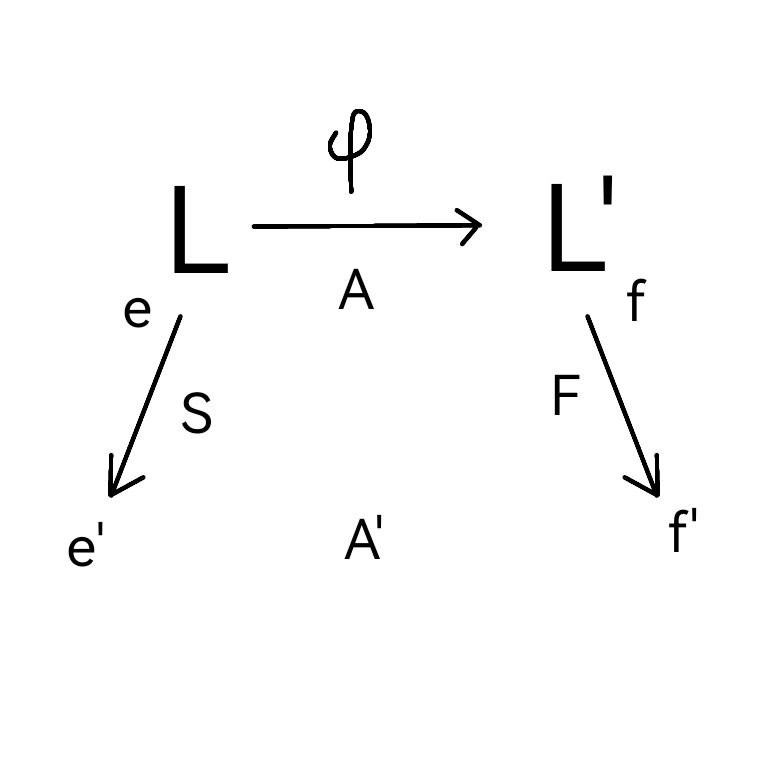
\includegraphics[width=1.0\linewidth]{images/6-7_1.png}
\end{wrapfigure}
    \tab\\
\begin{theorem}
    Пусть $\phi : L \longrightarrow L'$, e и f $-$ базисы в $L$ и $L'$ соответственно, y = Ax. Тогда $A' = F^{-1}AS$.
\end{theorem}
\tab\\\tab\\

\begin{proof}
\[
x = Sx'; y = Fy'
\]
\[
\begin{cases}
    y' = F^{-1}y = F^{-1}Ax = F^{-1}ASx'\\
    y' = A'x'\\
\end{cases} \Longrightarrow A' = F^{-1}AS
\]
\end{proof}

Если изначальные базисы e и f совпадают, то $l = L'$, S = F $\Longrightarrow$ $A' = S^{-1}AS$.\\

\begin{proposition}
    Пусть $\phi : L \longrightarrow L'$, rg $\phi$ = r. Тогда существуют базисы e, f :
    \[
    A_{\phi} = \begin{pmatrix}
        E_r & | & 0\\
        \hline
        0 & | & 0\\
    \end{pmatrix}
    \]
\end{proposition}
\begin{proof}
    dim Ker $\phi$ = n - r $-$ базис в ядре. Пусть он задан векторами $e_{r + 1}, ..., e_n$, $\phi(e_{r + 1} = ... = \phi(e_n) = 0$. Дополним $e_{r + 1}, ..., e_n$ до базиса в L векторами $e_1, ..., e_r$, тогда $\phi(e_1), ..., \phi(e_r)$ $-$ линейно независимый набор.\\
    Пусть $\phi(e_1) = f_1$, $\phi(e_2) = f_2$, ..., $\phi(e_r) = f_r$. Тогда $f_1, ..., f_r$ $-$ дополнение до базиса в $L'$ $-$ независимо от дополнения, корректный базис, требуемый нам.
\end{proof}

\begin{definition}
    Пусть $\phi: L \longrightarrow L'$ $-$ \textit{линейное отображение}.  Рассмотрим все такие отображения. На этом множеcтве M можно ввести следующие \textit{операции}
    \[
    \forall A, B \in M, \forall \alpha \in \mathbb{R}
    \]
    \[
    (A + B)(x) := A(x) + B(x)
    \]
    \[
    (\alpha A)(x) := \alpha A(x)
    \]
\end{definition}

\begin{definition}
   \textit{Композицией} линейных отображений А и В называется последовательное применение этих отображений, обозначается как ВА.
\end{definition}

По теореме о ранге, rg BA $\leq$ rg A и rg BA $\leq$ rg B.\\

Ранг отображения не превосходит размерности отображаемого пространства.\\

\section{Линейные преобразования($\phi:L\longrightarrow L)$}

По умолчанию dim L = n, базис в L $-$ e; y = Ax, $e \longrightarrow e'$ $\Longrightarrow$ $A' = S^{-1}AS$.\\

\begin{definition}
    Матрицы А и В называются \textit{перестановочными}, если АВ = ВА.
\end{definition}
\begin{itemize}
    \item AE = EA
    \item $AA^{-1}$ = $A^{-1}A$
    \item AA = AA
\end{itemize}

\begin{definition}
    Пусть задана матрица А. Тогда ее \textit{степенью} называется $k \in \mathbb{N} : \\A^k = A \cdot A \cdot ... \cdot A$ $-$ k раз, $A^0 = E$.
\end{definition}

\begin{definition}
    Пусть A --- матрица. Тогда
    \[
    P(A) = \alpha_0E + \alpha_1A + \alpha_2A^2 + ... + \alpha_kA^k
    \]
    --- \textit{многочлен преобразования}.
\end{definition}

Пусть $P_1(A)$ и $P_2(A)$ --- многочлены преобразования. Тогда $P_1P_2(A) = P_2P_1(A)$.

\begin{definition}
    Подпространство $L_1 \subset L$ называется \textit{инвариантным} относительно $\phi$, если 
    \[
    \forall x \in L_1 \tab \phi(x) \in L_1 \text{, или, что то же, } \phi(L_1) \subset L_1
    \]
\end{definition}
\begin{itemize}
    \item L инвариантно относительно любого $\phi$
    \item $\{0\}$ инвариантно относительно любого $\phi$
\end{itemize}

Пусть задано $\phi$. Тогда 
\begin{enumerate}
    \item
    \[
    L_1 = Ker\thinspace\phi \text{ --- инвариантно} (\forall x \in L_1 \hookrightarrow \phi(x) = 0 \in L_1)
    \]
    \item 
    \[
    L_2 = Im\thinspace\phi \text{ --- инвариантно} (\forall x \in L_2 \hookrightarrow \phi(x) \in L_2)
    \]
\end{enumerate}

Пусть $\phi : L \longrightarrow L'$ --- линейное преобразование. Пусть $e_1, ..., e_k$ --- базис в $L_1$, $e_{k + 1}, ..., e_n$ --- дополнение до базиса L.
\[
x \in L_1 \Longrightarrow x = \alpha_1e_1 + ... + \alpha_ke_k
\]
\[
\phi(x) = \alpha_1\phi(e_1) + ... + \alpha_k\phi(e_k) = \beta_1e_1 + ... + \beta_ke_k
\]
$\Longrightarrow$ все координаты, начиная с k + 1, равны 0 и у x, и у $\phi(x)$.

\begin{center}
    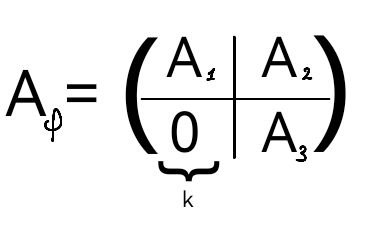
\includegraphics[width=0.25\linewidth]{images/6-7_2.png}
\end{center}

Если матрица имеет вид 
\[
\begin{pmatrix}
    k \times k & | & A_2\\
    \hline
    0 & | & A_3\\
\end{pmatrix}
\]
--- матрица преобразования $\phi : L \longrightarrow L'$, то $L_1 = <e_1, ..., e_k>$ --- инвариантно относительно $\phi$.\\

Аналогично: пусть $e_{n - m + 1}, ..., e_n$ --- базис в инвариантном подпространстве, тогда
\begin{center}
    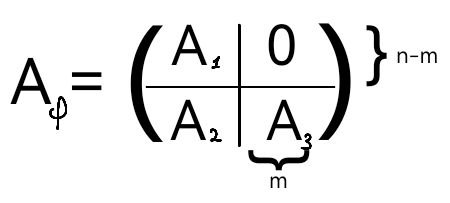
\includegraphics[width=0.25\linewidth]{images/6-7_3.png}
\end{center}

Пусть $e_{k + 1}, ..., e_{k + s}$ --- базис в ивариантном отношению $\phi$ подпространстве, тогда
\begin{center}
    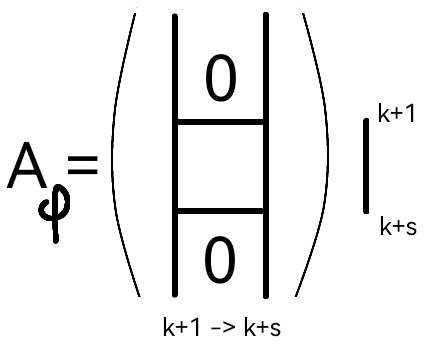
\includegraphics[width=0.25\linewidth]{images/6-7_4.png}
\end{center}

\begin{definition}
    Матрица преобразования, в которой от нуля отличаются только элементы квадратных клеток порядков $k_1, ..., k_m$ на диагонали, называется клеточно-диагональной.
\end{definition}
\[
L = L_1 \oplus ... \oplus L_m\thinspace\Longleftrightarrow\thinspace\begin{pmatrix}
    A_{k_1\times k_1} & 0 & ... & 0\\
    0 & A_{k_2\times k_2} & ... & 0\\
    ... & ... & ... & ...\\
    0 & 0 & ... & A_{k_m\times k_m}\\
\end{pmatrix}
\]

\section{Задача о собственных векторах}

\begin{definition}
    Преобразование $A$, сопоставляющее каждому вектору из инвариантного подпространства $L'$ вектор из $L'$, называется \textit{ограничением} $A$ на $L'$.
\end{definition}

\begin{theorem}
    Пусть А и В --- перестановочные линейные преобразования. Тогда ядро и образ одного из них инвариантно относительно другого.
\end{theorem}
\begin{proof}
\tab\\
    \begin{enumerate}
        \item $x \in Ker\thinspace A \Longrightarrow A(x) = 0 \Longrightarrow B(A(x)) = 0.$ Тогда $A(B(x)) = 0 \Longrightarrow B(x) \in Ker\thinspace A\newline \forall x \in Ker\thinspace A$.
        \item Если $x \in Im\thinspace A \Longrightarrow \exists$ вектор $z : x = A(z)$. Тогда $B(x) = B(A(z)) = A(B(z)) \Longrightarrow B(x) \in Im\thinspace A \tab \forall x \in Im\thinspace A.$
    \end{enumerate}
\end{proof}

$A$ и $A - \lambda E$ --- перестановочные как многочлены от $A$.\\

$Ker\thinspace(A - \lambda E)$ --- инвариантно относительно $A$.\\

\begin{definition}
    Пусть для некоторого $\lambda$ и для А, $Ker\thinspace(A - \lambda E)$ --- ненулевое. Тогда $\lambda$ --- \textit{собственное значение} А, $Ker\thinspace(A - \lambda E)$ --- \textit{собственное подпространство} А, соответствующее собственному значению $\lambda$.
\end{definition}

Рассмотрим частный случай. Пусть $Ker\thinspace (A - \lambda E) \neq \{0\}$. Тогда $\exists x \neq 0 : (A - \lambda E) = 0 \Longrightarrow Ax = \lambda Ex = \lambda x$. В таком случае если $\lambda = 0$, то $x \in Ker\thinspace A$.\\
При $\lambda \neq 0 : Ax = \lambda x$ --- гомотетия.

\begin{definition}
    Пусть х --- ненулевой вектор такой, что $Ax = \lambda x$. Тогда х называется \textit{собственным вектором}, соответствующим собственному значению $\lambda$.
\end{definition}

Пусть $x \neq 0$, $Ax = \lambda x$. Тогда $A(kx) = kAx = k\lambda x = \lambda(kx)$.

\begin{theorem}
    Собственные вектора и только они являются базисами одномерных инвариантных подпространств.
\end{theorem}
\begin{proof}
    \tab\\
    \begin{enumerate}
        \item Пусть вектор х --- собственный а $y$ принадлежит одномерному подпространству  $L'$ с базисом $x$. Тогда $y = \alpha x$ и $Ay = \alpha Ax = \alpha\lambda x \Longrightarrow Ay \in L'$.
        \item Пусть $x$ --- базис инвариантного подпромтранства $L'$. Тогда $Ax$ лежит в $L'$ и раскладывается по базису: $Ax = \lambda x$. Т.к. $x \neq 0$, он собственный.
    \end{enumerate}
\end{proof}

\underline{Как искать?}\\
\[
Ker\thinspace(A - \lambda E) \neq \{0\} \Longleftrightarrow det\thinspace(A - \lambda E) = 0 \longrightarrow
\]
\[
\longrightarrow \text{решаем} (A - \lambda E)x = 0 \longrightarrow \text{получаем собственные вектора.}
\]

\subsection{Характеристическое уравнение}

Пусть $\phi : L \longrightarrow L$, e --- базис, $A\phi = A$.\\

\begin{definition}
    det $(A - \lambda E)$ --- \textit{характеристическое уравнение}, его корни --- \textit{характеристические числа}.
\end{definition}

\[
\begin{pmatrix}
    a_{11} - \lambda & a_{12} & a_{13} & ... & a_{1n} \\
    a_{21} & a_{22} - \lambda & a_{23} & ... & ...\\
    ... & ... & ... & ... & ... \\
    a_{n1} & ... & ... & ... & a_{nn} - \lambda \\
\end{pmatrix}
\]

 $p(\lambda) = (-\lambda)^n + ...$ --- характеристический многочлен А. p(0) = det A --- свободный член.\\


 \underline{Какой коэффициент при $\lambda^{n - 1}$?}\\

$(a_{11} - \lambda)(a_{22} - \lambda) ... (a_{nn} - \lambda)$ --- любое другое слагаемое содержит  не более n - 2 "скобочек" с $\lambda$ $\Longrightarrow$ $\lambda^{n - 1}(-a_{11} - ... - a_{nn}) = -\lambda^{n - 1}(a_{11} + ... + a_{nn})
$ --- след матрицы А.\\


\subsection{Изменение характеристического уравнения при смене базиса}

Пусть е --- старый базис, $e'$ --- новый, S --- матрица перехода.

\[
p'(\lambda) = det\thinspace (A' - \lambda E) = 0
\]
\[
det\thinspace (A' - \lambda E) = det\thinspace (S^{-1}AS - \lambda S^{-1}ES) = det\thinspace (S^{-1}(A - \lambda E)S) = 
\]
\[
= det\thinspace (S^{-1}) \cdot det\thinspace (A - \lambda E) \cdot det\thinspace (S) = det\thinspace (A - \lambda E)
\]
--- инвариант, т.е. не зависит от базиса $\Longrightarrow$ $p(\lambda)$ --- характеристический многочлен преобразования. Тогда для линейного преобразования $\phi : L \longrightarrow L \hookrightarrow$ при переходе от е к $e'$, где А и $A'$ --- соответствующие матрицы преобразования в этих базисах
\[
det\thinspace A = det\thinspace A'
\]
\[
tr\thinspace A = tr\thinspace A'
\]


Пусть
\begin{figure}[h]
    \centering
    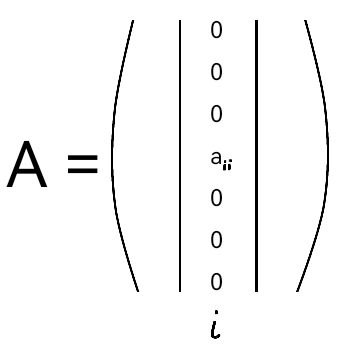
\includegraphics[width=0.3\linewidth]{images/6-7_6.png}
\end{figure}

Тогда $\phi(e_i) = a_{ii}e_i$.\\
Если существует базис из собственных векторов векторов, то А = diag ($\lambda_1, ..., \lambda_n$), где $\lambda_1, ..., \lambda_n$ --- собственные значения.


\begin{theorem}
    Пусть есть собственное инвариантное подпространство с различными $\lambda$, тогда их сумма --- прямая $\Longleftrightarrow$ собственные векторы,отвечающие разным собственным значениям, линейно независимы.
\end{theorem}
\begin{proof}
\tab\\
    $x_1\thinspace...\thinspace x_k$ --- разложение собственного вектора (\\
    $\downarrow\tab \downarrow$\\
    $\lambda_1\thinspace...\thinspace \lambda_k$ --- разложение собственного значения из определения не равны 0)\\
    $B_i = A - \lambda_i E$
    
    \[
        B_i(x_j) = Ax_j - \lambda_i Ex_j = (\lambda_j - \lambda_i)x_i = \begin{cases}
        0,\tab i = j\\
        \neq 0, \tab i\neq j\\
    \end{cases}
    \]

    Пусть л.з., тогда 
    \[
    \begin{cases}
        \exists x_k = \alpha_1x_1 + ... + \alpha_{k - 1}x_{k - 1}\\
        B_1B_2...B_{k - 1}(x_k) = (\lambda_k - \lambda_{k - 1})...(\lambda_k - \lambda_1)x_k, \text{ где }(\lambda_k - \lambda_{k - 1})...(\lambda_k - \lambda_1) \neq 0\\
        B_1B_2...B_{k - 1}(x_i) = 0,\thinspace i \in \{1, ..., k - 1\}
    \end{cases} \Longrightarrow
    \]
    $x_k = 0$, т.е. он не является собственным векором.
\end{proof}

\begin{theorem}
    Пусть $\phi: L \longrightarrow L$, $p(\lambda)$ --- характеристический многочлен.\\
    Пусть $p(\lambda) = (\lambda - \lambda_0)^S Q(\lambda)$, $\Q(\lambda_0) \neq 0$, $L_1$ --- собственное подпространство, соответствующее $\lambda_0$. Тогда
    \[
    1 \leq dim\thinspace L_1 \leq S
    \]
\end{theorem}
\begin{proof}
    Пусть $L_1$ --- собственное подпространство размерности k. Выберем базис: $e_1, ..., e_k$ --- базис в $L_1$. Произвольно дополним до базиса в L.
    \[
    A = \begin{pmatrix}
        \lambda_0 & ... & 0 & | & &\\
        ... & \lambda_0 & ... & | & &\\
        0 & ... &\lambda_0 & | & A_1 &\\
        0 & ... & 0 & | & &\\
        ... & ... & ... & | & &\\
    \end{pmatrix}\tab det(A - \lambda E) = (\lambda - \lambda_0)^kR(\lambda) = (\lambda - \lambda_0)^SQ(\lambda)
    \]
    $\phi(e_1) = \lambda_0e_1$\\
    ...\\
    $\phi(e_n) = \lambda_0e_n$\\
    k --- геометричская кратность, S --- алгебраическая кратность.
\end{proof}

\tab\\

\underline{Пример:} k < S\\

\[
A = \begin{pmatrix}
    1 & 1\\
    0 & 1\\
\end{pmatrix} \tab det\thinspace (A - \lambda E) = det\thinspace\begin{pmatrix}
    1 - \lambda & 1\\
    0 & 1 - \lambda\\
\end{pmatrix} = (1 - \lambda)^2 = 0
\]
$\Longrightarrow \lambda_{1,\thinspace 2} = 1$ --- корень кратности 2
\[
(A - \lambda E)x = \begin{pmatrix}
    0 & 1\\
    0 & 0
\end{pmatrix}x = 0 \Longrightarrow x = \begin{pmatrix}
    1\\
    0\\
\end{pmatrix}
\]

В случае $\lambda \in \mathbb{C}$, если $\lambda$ --- корень кратности $t$, то $\overline{\lambda}$ --- тоже корень кратности $t$.

\begin{theorem}
    Пусть $\lambda, \overline{\lambda}$ --- корни характеристического множества пространства $A$. Тогда им соответствуют ненулевое инвариантное подпространство $L_1$ такое, что через любой его ненулевой вектор проходит 2-мерное инвариантное подпрространство и $L_1$ не содержит собственных векторов.
\end{theorem}
\begin{proof}
$\lambda$, $\overline{\lambda} \longrightarrow x^2 + px + q = 0$, где $\lambda$, $\overline{\lambda}$ --- его корни.\\
\[
B = A^2 + pA + qE
\]
Докажем, что $L_1 = Ker\thinspace\phi$ --- искомое.\\
\[
B = (A - \lambda E)(A - \overline{\lambda}E)
\]
det B = 0, т.к. det $(A - \lambda E)$ = 0\\
Почему в $L_1$ нет собственных векторов?\\
Пусть h --- собственный вектор из $L_1$ $\Longrightarrow$ Bh = 0 $\Longrightarrow$ $(A^2 + pE + qE)h = (\lambda^2 + p\lambda + q)(h) = 0$ $\Longrightarrow$ h = 0 --- не является собственным вектором, противоречие.\\
Пусть $x \in L_1$, $<x, A(x)>$ --- л.н.з., т.к. иначе х --- собственный вектор, но, как было доказано выше, в $L_1$ нет собственных векторов.
\[
B(x) = A^2(x) + p(A(x)) + qEx = 0
\]
\[
A^2(x) = -pA(x) - qEx \Longrightarrow A(\alpha x + \beta (A(x))) = \widetilde{\alpha} + \widetilde{\beta}A(x)
\]
\end{proof}









\section{Диагонализируемость}

\begin{proposition}
    У линейного преобразования существует либо одномерное собственное подпространство, либо инвариантное двумерное.
\end{proposition}

\begin{lemma}
    Если пространство имеет нечетную размерность, то унего существует одномерное собственное подпространство.
\end{lemma}
\begin{proof}
$p(\lambda)$ --- нечетная степень, 1 коэффициент равен -1 $\Longrightarrow$ существует вещественный корень, которому соответствует собственный вектор $\Longrightarrow$ ему можно сопоставить собственное подпространство.    
\end{proof}

Если имеется базис из собственных векторов преобразования $\phi$ $e_1, ..., e_n$, то в этом базисе
\[
A_{\phi} = diag(\lambda_1, ..., \lambda_n),\tab\phi(e_i) = \lambda_ie_i
\]
\begin{definition}
    Если существует базис, в котором матрица преобразования диагональная, то оно \textit{диагонализируемо}.
\end{definition}

\begin{theorem}[Критерий диагонализируемости]
    Пусть заданы $L$, $\phi$.\\
    $\phi$ --- диагонализируемо $\Longleftrightarrow$ $L = L_1\oplus ... \oplus L_k$, где $L_i$ --- собственное подпространство.
\end{theorem}
\begin{proof}
    \tab\\
    $\Longrightarrow$\\
    $\phi$ диагонализируемо, значит существует базис, в котором $A_{\phi} = diag(\lambda_1, ..., \lambda_k)$. Упорядочим $\lambda_1 \leq ... \leq \lambda_k$, т.е. каждому $\lambda_i$ соответствует собственное $L_i$, т.к. объединение --- прямая сумма.\\
    \tab\\
    $\Longleftarrow$\\
    В каждом подпространстве выбираем базис, объединение базисов --- базис пространства $\Longrightarrow$ $A_{\phi}$ имеет нужный вид.
\end{proof}

\begin{theorem}[Необходимое условие диагонализируемости]
    Пусть заданы $L$, $\phi$.\\
    Все корни характеристического многочлена $p(\lambda)$ --- вещественные.
\end{theorem}
\begin{proof}
Пусть задан корень характеристического многочлена $\lambda_i \in \mathbb{R}$, кратности $\alpha_i$. Тогда ему соответствует собственное подпространство такое, что $1 \leq dim L_i \leq \alpha_i$.

Пусть задан корень характеристического многочлена $\lambda_i \in \mathbb{C}$ $\Longrightarrow$ сумма кратностей вещественных корней меньше размерности пространства $\Longrightarrow$ не диагонализируемо.
\end{proof}

\begin{theorem}[Достаточное условие диагонализируемости]
    Пусть заданы $L$, $\phi$.\\
    Все корни характеристического многочлена $p(\lambda)$ --- вещественные и различные.\\

    Собственные векторы, отвечающие различным собственным значениям линейно независимы, значит можно выбрать в качестве базиса собственные векторы диагонализируемого пространства.\\

    \underline{Матричная формулировка:} Пусть у квадратной матрицы А все собствнные значения веществнны и различны $\Longrightarrow$ 
    \[
    \exists S : S^{-1}AS = diag
    \]
\end{theorem}
\begin{proof}
    Т.к. матрица квадратная, ей можно поставить в соответствие преобразование $\phi$. Из необходимого условия, все корни характеристического многочлена преобразования вещественные. Если они все различные, то матрицу преобразования можно представить в диагональном виде $\Longrightarrow$ $\phi$ диагонализируемо.
\end{proof}

Критерий диагонализируемости $\Longleftrightarrow$ все $\lambda_1, ...., \lambda_n$ --- вещественные и $\forall \lambda_i$ кратности $\alpha_i$ размерность собственного подпространства равна $\alpha_i$.

\begin{theorem}[Гамильтона-Кэли]
    Рассмотрим характеристический многочлен $p(\lambda) = det(A - \lambda E)$. Тогда
    \[
    p(A) = 0
    \]
\end{theorem}
\begin{proof}
Матрица $A - \lambda E$ почти всегда невырождена. Считаем, что $\lambda$ не являетсяя корнем характеристического уравнения  $\Longrightarrow$ обратная матрица:
\[
(A - \lambda E)^{-1} = \dfrac{1}{det(A - \lambda E)}B(\lambda)\eqno{(*)}
\]
где $B(\lambda)$ --- элементы-многочлены степени $\leq$ n - 1.
\[
B(\lambda) = B_0 + B_1\lambda + ... + B_{n - 1}\lambda^{n - 1}
\]
Умножим (*) на $(A - \lambda E) det (A - \lambda E)$:
\[
E\cdot p(\lambda) = B(\lambda)(A - \lambda E)
\]
\[
p(\lambda) = a_0E + a_1\lambda E + ... + a_n \lambda^nE = (B_0 + B_1\lambda + ... +B_n\lambda^n)(A - \lambda E)
\]
$\lambda^0 = a_0E = B_0A$\\
$\lambda^1 = a_1E = B_1A - B_0E\tab|\cdot A$\\
$\lambda^2 = a_2E = B_2A - B_1E\tab|\cdot A^2$\\
...\\
$\lambda_n = a_nE = -B_{n - 1}E\tab|\cdot A^n$\\
Сложим и получим:
\[
0 = a_0E + a_1EA + ... = p(A)
\]
\end{proof}

\section{Линейны функции}

\begin{definition}
    f - \textit{линейная функция}, если 
    \begin{enumerate}
        \item $\forall x, y\in L \hookrightarrow f(x + y) = f(x) + f(y)$
        \item $\forall x\in L \forall \alpha \in \mathbb{R} \hookrightarrow f(\alpha x) = \alpha f(x)$
    \end{enumerate}
\end{definition}

\begin{definition}
    Пусть задан базис $e$. Тогда
    \[
    f(x) = f(x_1e_1 + ... + x_ne_n) = x_1f(e_1) + ... + x_nf(e_n) = (f(e_1), ..., f(e_n))\begin{pmatrix}
        x_1\\
        ...\\
        x_n\\
    \end{pmatrix} = \phi_ex
    \]
    где $(f(e_1), ..., f(e_n)) = \phi_e$ --- \textit{компоненты функции}, или \textit{координатна строка}. Функция однозначно задается $\phi_e$ в базисе $e$.
\end{definition}

Для перехода между базисами верно, что
\[
A' = P^{-1}AS \tab \Longrightarrow \tab \phi_e' = P^{-1}\phi_eS
\]
Для действительных чисел
\[
A' = AS \tab \Longrightarrow \tab \phi_e' = \phi_eS
\]

Пусть $M$ --- множество всех линейных функций, заданных на $L$. Введем сумму линейных функций
\[
\forall f_1, f_2 \in M \forall x \in L \hookrightarrow (f_1 + f_2)(x) = f_1(x) + f_2(x)
\]
и умножение линейной функции на число
\[
\forall f \in M \forall \alpha \in \mathbb{R} \forall x \in L \hookrightarrow (\alpha f)(x) = \alpha f(x)
\]
Таким образом, $M$ --- линейное пространство, причем если в $L$ выбран базис $e$, то любая функция из $M$ задается координатной строкой в этом базисе.

В сумме функций координатные строки складываются. Если умножить функцию на число, координатная строка умножится на это число $\Longrightarrow$ $M$ изоморфно пространству строк длины n со стандартными операциями, т.е. пространство $L$ размерности n переходит в n-мерное пространство линейных функций на $L$. Это пространство называют \textit{сопряженным} к $\L$ --- $L^*$.

Если $L$ имеет базис $e$, а $L^*$ базис $f$, то $f$ взаимен с $e$, если
\[
f_i(e_j) = \begin{cases}
    0,\tab i\neq j\\
    1,\tab i = j\\
\end{cases}
\]
Существует $L^* \longrightarrow L^{**}$.

\begin{theorem}
    $L^{**}$ может быть сопоставлено $L$.
\end{theorem}

\begin{definition}
    Пусть дано $L$, $B(x, y)$ --- функция такая, что $\forall x, y \in L\thinspace B(x, y) \in \mathbb{R}$. $B(x, y)$ называется \textit{билинейной}, если выполнена линейность по 2 аргументам, т.е.
    \[
    \forall x, y \in L \hookrightarrow B(x + y, z) = B(x, z) + B(y, z)
    \]
    \[
    \forall x, y \in L \forall \alpha \in \mathbb{R} \hookrightarrow B(\alpha x, y) = \alpha B(x, y)
    \]
    и
    \[
    \forall x, y \in L \hookrightarrow B(x, y + z) = B(x, y) + B(x, z)
    \]
    \[
    \forall x, y \in L \forall \alpha \in \mathbb{R} \hookrightarrow B(x, \alpha y) = \alpha B(x, y)
    \]
\end{definition}

Пусть задано пространство $L_n$, $e$ --- базис, $x = \begin{pmatrix}
    x_1\\
    ...\\
    x_n\\
\end{pmatrix}$, $y = \begin{pmatrix}
    y_1\\
    ...\\
    y_n\\
\end{pmatrix}$. Тогда
\[
B(x, y) = B(x_1e_1 + ... + x_ne_n, y_1e_1 + ... + y_ne_n) = \sum_{i, j = 1}^n x_iy_j B(e_i, e_j) = 
\]
\[
=\begin{pmatrix}
    x_1 & ... & x_n\\
\end{pmatrix}\begin{pmatrix}
    B(e_1, e_1) & ... & B(e_1, e_n)\\
    ... & ... & ... \\
    B(e_n, e_1) & ... & B(e_n, e_n)\\
\end{pmatrix}\begin{pmatrix}
    y_1\\
    ...\\
    y_n\\
\end{pmatrix} = x^TBy
\]

Биленейная функция $\Longleftrightarrow$ биленейная форма.












\section{Билинейные и квадратичные формы}

Для $B' = S^TBS$ верно, что
\begin{enumerate}
    \item $det\thinspace B' = (det\thinspace S)^2det\thinspace B$ $\Longrightarrow$ знак не меняется
    \item $, S^T$ --- невырожденные $\Longrightarrow$ $rg\thinspace B' = rg\thinspace B$
\end{enumerate}

\begin{definition}
    Пусть $b(x, y)$ --- симметричная билинейная форма в базисе $e$. Тогда \textit{квадратичной формой} называется
    \[
    k(x) = b(x, x) = x^TBx,
    \]
    где B --- матрица квадратичной формы в базисе $e$.
\end{definition}

Для k(x + y) верно, что
\[
k(x + y) = b(x + y, x + y) = b(x, x) + b(x, y) + b(y, x) + b(y, y)
\]

При этом существует и единственна  симметричная биленейная форма, порождающая данную квадратичную.

\begin{definition}
    Квадратичная форма k(x) в базисе $e$ имеет \textit{диагональный} вид, если
    \[
    k(x) = \sum_{i = 1}^n\alpha_ix_i^2
    \]
    В этом базисе матрица квадратичной формы диагональна.
\end{definition}

\begin{definition}
    Квадратичная форма k(x) в базисе $e$ имеет \textit{канонический} вид, если
    \[
    k(x) = \sum_{i = 1}^n\alpha_ix_i^2, \tab \alpha_i = \pm 1, 0
    \]
\end{definition}

\begin{theorem}
    Для любой квадратичной формы существует базис, в котором она имеет диагональный вид.
\end{theorem}
\begin{proof}
Пусть имеется квадратичная форма k(x) и ее матрица в некотором базисе В. Применим к В последовательность эоементарных преобразований. На первом этапе возможны случаи:
\begin{enumerate}
    \item $b_{11} \neq 0$ $\Longrightarrow$ вычитаем первую строку, умноженную на $\dfrac{b_{i1}}{b_{11}}$ для i-ой строки, из всех нижележащих строк. Аналогично вычитаем первый столбец. Матрица В переходит в 
    \[
    B_1 = \begin{pmatrix}
        b_{11}' & 0 & ...0\\
        0 & & & \\
        ... & C_1 & & \\
        0 & & & \\
    \end{pmatrix}
    \]
    где $C_1$ --- симметрическая квадратная матрица порядка n - 1.
    \item $b_{11} = 0$ --- особый случай.
    \begin{itemize}
        \item $b_{1i} = 0 \forall i = 2, ..., n$ $\Longrightarrow$ матрица уже имеет вид $B_1$.
        \item $\exists i : b_{1i} \neq 0$. Приведем матрицу к виду $B_1$ с помощью вспомогательного преобразования:если $b_{ii} \neq 0$, то i-ая строка переставляется с первой и i-ый столбец переставляется с первым; если $b_{ii} = 0$, то i-ая строка прибавляется к первой и i-ый столбец прибавляется к первому.
    \end{itemize}
\end{enumerate}
Пусть после k шагов матрица имеет вид
\[
B_k = \begin{pmatrix}
    b_{11}' & &  & | & &\\
    ... & ... & ... & | & 0 & \\
     & & b_{kk}' & | & & \\
    - & - & - & | & - & - \\
     & 0 & & | & C_k & \\
\end{pmatrix}
\]
где $C_k$ --- симметрическая матрица порядка n - k.
После (n - 1) шага матрица $C_{n - 1}$ имеет порядок 1, а В имеет вид
\[
B' = \begin{pmatrix}
    b_{11}' & ... & ...\\
    ... & ... & ... \\
    ... & ... & b_{nn}'\\
\end{pmatrix}
\]
Итого $B' = S^TBS$, где $S = S_1...S_n$ $\Longrightarrow$ существует базис, в котором форма имеет канонический вид.
\end{proof}

\begin{definition}
    \textit{Ранг квадратичной формы} --- количество $\pm 1$ на диагонали матрицы в каноническом виде, равен рангу В.
\end{definition}

\begin{definition}
    Квадратичная форма k(x) \textit{положительно определена} на $L_1$, если
    \[
    \forall x \in L_1, x \neq 0 \hookrightarrow k(x) > 0
    \]
    Квадратичная форма k(x) \textit{положительно полуопределена} на $L_1$, если
    \[
    \forall x \in L_1, x \neq 0 \hookrightarrow k(x) \geq 0
    \]
    Аналогично для \textit{отрицательной} определенности и полуопределенности.\\
    Если форма положительно/отрицательно полуопределена/определена, то она называется \textit{знакоопределенной}, иначе \textit{знаконеопределенной}.
\end{definition}


\begin{table}[h]
    \centering
    \begin{tabular}{|c|c|}
        \hline
        Знакоопределенность & Канонический вид\\
         \hline
        k(x) > 0 & diag(1, ..., 1)\\
         \hline
        k(x) $\geq$ 0 & diag(1 и 0)\\
         \hline
        k(x) < 0 & diag(-1, ..., -1)\\
         \hline
        k(x) $\leq$ 0 & diag(-1 и 0)\\
         \hline
        знаконеопределенность & diag(и 1, и -1)\\
         \hline
    \end{tabular}
\end{table}

\begin{theorem}[Закон инерции квадратичных форм]
    В любом базисе, в котором форма имеет канонический вид, количество "+1" и "-1" на диагонали постоянно.
\end{theorem}

\begin{definition}
    Пусть $L^{(-)} \subset L$ --- пространство максимальной размерности, где k(x) < 0. Эту размерность назовем \textit{отрицательным индексом инерции}. Аналогично определяется \textit{положительный индекс инерции}.
\end{definition}

\begin{lemma}
    Отрицательный индекс инерции равен количеству "-1" в каноническом виде, аналогично положительный индек равен количеству "+1".
\end{lemma}
\begin{proof}
    Пусть r = rg k(x).\\
    Пусть $k(x) = -x_1^2 - x_2^2 - ... - x_k^2 + x_{k + 1}^2 + ... + x_r^2 + 0\cdot x_{r + 1}^2 + ... + 0\cdot x_n^2$\\
    \[
    L_1 = <e_1, ..., e_k>\tab L_2 = <e_{k + 1}, ..., e_n>\tab L_1 \oplus L_2 = L
    \]
    k(x) --- отрицательно определена на $L_1$ $\Longrightarrow$ $dim\thinspace L^{(-)} \geq k$\\
    k(x) --- положительно определена на $L_2$.\\
    Пусть $L^{(-)}$ таково, что $dim\thinspace L^{(-)} > k$. Тогда
    \[
    L^{(-)} \cap L_2 :
    \]
    \begin{enumerate}
        \item $dim\thinspace L^{(-)} + dim\thinspace L_2 > n$
        \item $\exists \widetilde{x} \neq 0 \in L^{(-)}$ --- $\begin{cases}
            k(\widetilde{x} \geq 0\\
            k(\widetilde{x} < 0
        \end{cases}$
    \end{enumerate}
    p --- положительный индекс, q --- отрицательный $\Longrightarrow$ rg = p + q.
\end{proof}

\begin{definition}
    \textit{Сигнатура} --- разность положительного и отрицательного индексов инерции.
\end{definition}

\begin{lemma}
    k(x) > 0 $\Longrightarrow$ в любом базисе диагональные элементы матрицы $b_{ii}$ > 0
    \[
    b_{ii} = b(e_i, e_i) = k(e_i) > 0
    \]
\end{lemma}
\begin{note}
    Обратное не верно, контрпример:
    \[
    \begin{pmatrix}
        1 & 2\\
        2 & 1\\
    \end{pmatrix} \text{ --- не является положительно определенной}
    \]
\end{note}

\begin{theorem}[Критерий Сильвестра]
\tab\\
    \begin{enumerate}
        \item k(x) > 0 $\Longleftrightarrow$ в любом базисе главные миноры матрицы больше 0.
        \item k(x) < 0 $\Longleftrightarrow$ главные миноры меняют знак: нечетные --- меньше 0, четные --- больше.
    \end{enumerate}
\end{theorem}
\begin{proof}
    \tab\\
    \begin{enumerate}
        \item $\Longrightarrow$\\
        Пусть k(x) > 0\\
        \[
        \begin{pmatrix}
            b_{11} & ...\\
            ... & ...\\
        \end{pmatrix}\tab \text{по лемме нет особого случая}\Longrightarrow
        \]
        \[
        \text{вычитаем только верхние строки из нижних}\begin{pmatrix}
            b_{11} & ... & 0\\
            ... & b_{22}' &...\\
            ... & ... & ...\\
        \end{pmatrix}, b_{ii}' > 0
        \]
        В каждом главном миноре выполняем только элементарные операции, которые не меняют det. Все $\Delta_i > 0$ и они не менялись.\\
        $\Longleftarrow$\\
        Пусть все главные миноры больше 0.\\
        \[
        \begin{pmatrix}
            b_{11} & 0 & ... & 0\\
            0 & b_{22}' & ... & 0\\
            ... & ... & ... & ...\\
            0 & ... & ... & 0\\
        \end{pmatrix}
        \]
        $b_{11} = \Delta_1 > 0$\\
        $\Delta_2 = b_{22}'b_{11} > 0$ $\Longrightarrow$ $b_{22}' > 0$\\
        ...\\
        Аналогично остальные $b_{ii}' > 0$.
        \item k(x) отрицательно определена $\Longleftrightarrow$ (-1)k(x) --- положительно определена.
        \[
        \begin{pmatrix}
            -1 & 0 & ... & 0\\
            0 & -1 & ... & 0\\
            ... & ... & ... & ...\\
            0 & ... & 0 & -1\\\
        \end{pmatrix}\tab det(-E_k) = (-1)^k
        \]
    \end{enumerate}
\end{proof}

\begin{proposition}[Достаточное условие знаконеопределенности k(x)]
    Если $\Delta_2 < 0$, то k(x) --- знаконеопределена.
\end{proposition}
\begin{proof}
    Пусть задана матрица B, $\Delta_2 < 0$, $L_1 = <e_1, e_2>$.\\
    На $L_1$ у k(x) матрица $\widetilde{B}$ \tab $|\widetilde{B}| = \Delta_2 < 0$\\
    Перейдем в канонический вид:
    \[
    \begin{cases}
        \widetilde{B'} = S^TBS\\
        |\widetilde{B}| < 0\\
    \end{cases} \tab det\thinspace\widetilde{B'} = (det\thinspace S)^2 det\thinspace\widetilde{B},
    \]
    где $(det\thinspace S)^2$ > 0, $det\thinspace\widetilde{B} = \Delta_2 < 0$
    \[
    det\thinspace\widetilde{B'} = \widetilde{b_{11}'}\widetilde{b_{22}'} < 0
    \]
    $\Longleftarrow$ в каноническом виде на диагонали содержатся и 1, и -1.
\end{proof}

\section{Евклидовы пространства}

\begin{definition}
    \textit{Евклидово пространство $\cal E$} --- линейное пространство, на котором введено скалярное произведение
    \[
    \forall x, y \in {\cal E} \hookrightarrow (x, y) \in \mathbb{R}
    \]
    \begin{enumerate}
        \item $\forall x, y \in {\cal E} \hookrightarrow (x, y) = (y, x)$
        \item $\forall x, y, z \in {\cal E} \hookrightarrow (x + y, z) = (x, z) + (y, z)$
        \item $\forall x, y \in {\cal E} \thinspace\forall \alpha \in \mathbb{R} \hookrightarrow (\alpha x, y) = \alpha(x, y)$
        \item  $\forall x \neq 0, x \in {\cal E} \hookrightarrow (x, x) > 0$
        \item[$4^*$] $\forall x \in {\cal E} \hookrightarrow (x, x) \geq 0$\\
        $(x,x) = 0 \Longleftrightarrow x = 0$
    \end{enumerate}
\end{definition}

Первые три свойства скалярного произведения порождают симметричную билинейную форму, а если добавить к ним 4, то они будут порождать положительно определенную квадратичную форму.

\begin{definition}
    \textit{Длина} вектора $x\in \cal E$
    \[
    |x| = \sqrt{(x, x)}
    \]
\end{definition}

\begin{definition}
    \textit{Угол} между векторами $x, y \in {\cal E} : x, y \neq 0$
    \[
    cos\thinspace(x^\wedge y) = \dfrac{(x, y)}{|x||y|}
    \]
\end{definition}

\begin{theorem}[Неравенство Коши-Буняковского (КБШ)]
    Пусть задано евклидово пространство $\cal E$, тогда $\forall x, y \in \cal E$ справедливо неравенство
    \[
    (x, y)^2 \leq (x, x) (y, y)
    \]
\end{theorem}

\begin{theorem}[Неравенство треугольника]
    Пусть задано евклидово пространство $\cal E$, тогда $\forall x, y \in \cal E$ справедливо неравенство
    \[
    |x + y| \leq |x| + |y|
    \]
\end{theorem}
\begin{proof}
    \[
    (x + y, x+ y) = |x|^2 + 2(x, y) + |y|^2 \leq \{ \text{т.к. из КБШ } |(x, y)| \leq |x||y| \} \leq |x|^2 + 2|x||y| + |y|^2 = (|x| + |y|)^2
    \]
    \[
    \Longrightarrow |x + y| \leq |x| + |y|
    \]
\end{proof}

\section{Ортогонализация}

\begin{definition}
   Будем говорить, что векторы х и у \textit{ортогональны}, если (х, у) = 0.
\end{definition}

\begin{corollary}
    Если вектор х ортогонален к любому вектору, то х = 0.
\end{corollary}

\begin{definition}
    Пусть дано $\cal E$ --- евклидово пространство, в нем задан базис $e_1, ..., e_n$. Тогда $(x,y) = x^T\text{Г}y$ и 
    \[
    \text{Г} = \begin{pmatrix}
        (e_1, e_1) & ... & (e_1, e_n)\\
        ... & ... & ...\\
        (e_n, e_1) & ... & (e_n, e_n)\\
    \end{pmatrix} \textit{ --- матрица Грама}
    \]
\end{definition}

\begin{theorem}
    Пусть задан некоторый набор векторов $f_1, ..., f_n$. $det\thinspace\text{Г}_f \geq 0$, причем
    \begin{enumerate}
        \item >0, если набор лнз
        \item =0, если набор лз
    \end{enumerate}
\end{theorem}
\begin{proof}
    $f_1, ..., f_k$ --- лз $\Longrightarrow$ существует нетривиальная линейная комбинация, равная нулю:
    \[
    \alpha_1f_1 + ... + \alpha_kf_k = 0, \tab \alpha_1^2 + ... + \alpha_k^2 > 0
    \]
    Домножим скалярно на $f_1, ..., f_k$
    \[
    \begin{cases}
        \alpha_1(f_1, f_1) + \alpha_2(f_1, f_2) + ... + \alpha_k(f_1, f_k) = 0\\
        \alpha_1(f_2, f_1) + \alpha_2(f_2, f_2) + ... + \alpha_k(f_2, f_k) = 0\\
        ...\\
        \alpha_1(f_k, f_1) + ... + \alpha_k(f_k, f_k) = 0\\
    \end{cases}
    \]
    Система линейно однородна, есть нетривиальное решение $\Longrightarrow$ det = 0.
\end{proof}

Докажем неравенство КБШ:
\begin{proof}
    \[
    det\begin{pmatrix}
        (x, x) & (x, y)\\
        (y, x) & (y, y)\\
    \end{pmatrix} \geq 0
    \]
    Отсюда получаем искомое, причем равенство $\Longleftrightarrow$ x и у --- линейно зависимые.
\end{proof}

При переходе к другому базису Г$' = S^T$ГS\\
В ОНБ Г = Е\\
Пусть базис $f_1, ..., f_n$ --- ортогональный, тогда
\[
x = \sum_{i = 1}^n{\dfrac{(x, f_i)}{|f_i|^2}\cdot f_i}
\]
\begin{theorem}[Равенство Парсеваля]
    \[
    (x, x) = |x|^2 = \sum_{i = 1}^n{\dfrac{(x, f_i)^2}{|f_i|^2}}
    \]
\end{theorem}

\begin{definition}
    Матрица $S$ --- \textit{ортогональная}, если $S^TS = E$. Для такой матрицы верно, что
    \begin{enumerate}
        \item $S^T = S^{-1}$ $\Longrightarrow$ $SS^T = E$
        \item $(det\thinspace S)^2 = 1$, $det\thinspace S = \pm 1$
    \end{enumerate}
\end{definition}

\begin{definition}
    Пусть $E_1 \subset E$, заданы базис и скалярное произведение Г, тогда $E_1^{\perp}$ --- \textit{ортогональное дополнение} к $E_1$. Это множество всех векторов $x \in E_1 : \forall y \in E\tab (x, y) = 01$
\end{definition}

$E_1^{\perp}$ является подпространством.

$\widetilde{x}, \widetilde{\widetilde{x}}$ ортогональны у $\Longrightarrow$ $\alpha\widetilde{x} + \beta\widetilde{\widetilde{x}}$ --- тоже ортогонально у, 
\[
(\alpha\widetilde{x} + \beta\widetilde{\widetilde{x}}, y) = \alpha(\widetilde{x}, y) + \beta(\widetilde{\widetilde{x}}, y) = 0 \text{, т.к. } (\widetilde{x}, y) = 0 \text{ и } (\widetilde{\widetilde{x}}, y) = 0, \tab 0 \in E_1^{}
\]

Кроме того, если dim E = n, dim $E_1$ = $k$, то dim $E_1^{\perp}$ = n - k

\begin{definition}
    Пусть $E_1, E_2$ --- подпространства E. $E_1$ и $E_2$ \textit{ортогональны}, если 
    \[
    \forall x \in E_1\thinspace \forall y \in E_2 \hookrightarrow (x, y) = 0
    \]
\end{definition}

Пусть $E_1 \subset E$, в $E_1$ выбран ортогональный базис $f_1, ..., f_k$. Найдем ортогональную проецию вектора x на $E_1$. Дополним до ортогонального базиса в E, добавив ортогональный базис $E_1^{\perp}$ $f_{k + 1}, ..., f_n$, тогда
\[
x = \alpha_1f_1 + ... + \alpha_kf_k + ... + \alpha_nf_n \text{, где } \alpha_1f_1 + ... + \alpha_kf_k \text{ --- проекция на } E_1 \Longrightarrow \alpha_i = \dfrac{(x_i, f_i)}{(f_i, f_i)} \Longrightarrow
\]
\[
x_{E_1}^{\perp} = \sum_{i = 1}^k{\dfrac{(x_i, f_i)}{(f_i, f_i)} \cdot f_i}
\]

Пусть $E_1 \subset E$, в $E_1$ = <$f_1, ..., f_k$>. Ортогонализуем базис в $E_1$.\\

\underline{Процесс ортогонализации Грама-Шмидта}\\
Положим $g_1 = f_1$. Далее из $f_2$ вычтем его ортогональную проекцию на линейную оболочку $g_1$, тогда
\[
g_2 = f_2 - \dfrac{(f_2, f_1)}{|g_1|^2}g_1
\]
Отметим, что $g_2$ раскладывается по $f_1 = g_1$ и $f_2$, причем $g_2 \neq 0$, т.к. в противном случае $f_1$ и $f_2$ были бы пропорциональны.

Продолжим таким же образом. Пусть построено k попарно ортогональных векторов $g_1, .., g_k$, тогда для k + 1:
\[
g_{k + 1} = f_{k + 1} - \sum_{i = 1}^k{\dfrac{(f_{k + 1}, g_i)}{|g_i|^2}g_i}
\]
Таким образом помтроим n векторов, которые будут попарно ортогональны, т.к. каждый (i+1)-ый вектор является проекцией $f_{i + 1}$ на ортогональное дополнение линейной оболочки $g_1, ..., g_k$. Кроме того $\forall i \in \{1, ..., n\}$ $g_i \neq 0$, т.к. иначе векторы были ьы линейно зависимы. Итого, построен ортогональный базис.

\section{Сопряженные преобразования}

\begin{definition}
    Преобразование $A^*$ называется \textit{сопряженным} к преобразованию А, если
    \[
    \forall x, y \in E \tab (A(x), y) = (x, A^*(y))
    \]
\end{definition}

\begin{theorem}
    Для любого преобразования А существует и единственно сопряженное преобразование $A^*$.
\end{theorem}
\begin{proof}
    \[
    x^TA^T\text{Г}e = (Ax)^T\text{Г}y = x^T\text{Г}A^*y \tab A^T\text{Г} = \text{Г}A^*
    \]
    Преобразование $A^* = \text{Г}^{-1}A^T\text{Г}$ подходит.
\end{proof}

\begin{theorem}
    \[
    Im\thinspace A = (Ker\thinspace A^*)^{\perp}
    \]
\end{theorem}
\begin{proof}
    \[
    \forall x \in E \tab y \in Ker\thinspace A^*
    \]
    \[
    (A(x), y) = (x, A^*(y)) = (x, 0) = 0 \Longrightarrow Im\thinspace A \subset (Ker\thinspace A^*)^{\perp}
    \]
    Обозначим dim E = n, rg A = r.
    \[
    dim (Ker\thinspace A^*) = dim (\text{пространства, являющегося решением } A^Ty = 0) = n - r
    \]
    \[
    dim (Ker\thinspace A^*)^{\perp} = n - (n - r) = r = dim\thinspace Im\thinspace A
    \]
\end{proof}


\section{Самосопряженные преобразования}

\begin{definition}
    Преобразование А называется \textit{самосопряженным}, если $A = A^*$, т.е.
    \[
    (A(x), y) = (x, A(y))
    \]
\end{definition}

Из определения сразу следует, что преобразование самосопряжено $\Longleftrightarrow$ матрица преобразования в ОНБ симметрична.

\begin{proposition}
    Все корни характеристического многочлена самосопряженного преобразования вещественны.
\end{proposition}
\begin{proof}
    Докажем от противного. Пусть у А $\exists \lambda \in \mathbb{C}$ --- корень характеристического многочлена $\Longrightarrow$ существует инвариантное двумерное подпространство $E_1$ без собственных векторов. Рассмотрим на нем А
    \[
    x \in E_1 \longrightarrow A(x) \in E_1
    \]
    Выберем ОНБ
    \[
    \widetilde{A} = \begin{pmatrix}
        \alpha & \beta \\
        \beta & \gamma \\
    \end{pmatrix}
    \]
    \[
    det (\widetilde{A} - \lambda E) = det \begin{pmatrix}
        \alpha - \lambda & \beta \\
        \beta & \gamma - \lambda \\
    \end{pmatrix} = (\alpha - \lambda)(\gamma - \lambda) - \beta^2 = 0
    \]
    Здесь все $\lambda$ --- комплексные, т.к. нет собственных векторов, но у $(\alpha - \lambda)(\gamma - \lambda) - \beta^2 = 0$ есть вещественные корни $\Longrightarrow$ противоречие.
\end{proof}

\begin{corollary}
    Все корни симметрической матрицы преобразования вещественны.
\end{corollary}

\begin{theorem}
    Собственные векторы, отвечающие различным собственным значениям самосопряженного преобразования попарно ортогональны.
\end{theorem}
\begin{proof}
    Пусть А --- самосопряженное, $h_1(\lambda_1)$, $h_1(\lambda_1)$, --- собственные вектора, отвечающие $\lambda_1$ и $\lambda_2$ соответственно.

    $(Ah_1, h_2) = (\lambda_1h_1, h_2) = \lambda_1(h_1, h_2)$\\
    $\tab||\tab\tab\tab\tab\tab||$\\
    $(h_1, Ah_2) = (h_1, \lambda_2h_2) = \lambda_2(h_1, h_2)$\\

    \[
    (\lambda_1 - \lambda_2)(h_1, h_2) = 0 \tab (\lambda_1 - \lambda_2) \neq 0 \Longrightarrow (h_1, h_2) = 0
    \]
\end{proof}

\begin{theorem}
    Пусть задано А --- самосопряженное преобразование Е, $E_1 \in E$ инвариантное относительно А. Тогда $E_1^{\perp}$ тоже инвариантно относительно А.
\end{theorem}
\begin{proof}
    \[
    \forall x \in E_1 \hookrightarrow A(x) \in E_1 \tab
    \]
    $A(x), y) = (x, A(y)) = 0$ $\Longrightarrow$ $A(y) \in E_1^{\perp}$
\end{proof}

\begin{theorem}
    Пусть задано А --- самосопряженное преобразование Е. Тогда в Е существует ОНБ из собственных векторов А.
\end{theorem}
\begin{proof}
    Пусть все собственные значения вещественные, $L_1, ..., L_k$ --- собственные подпространства, L = $L_1 \oplus ... \oplus L_k$. Докажем, что E = L.

    Допустим обратное. Тогда L --- инвариантно, dim L < dim E
    
    $L^\perp$ тоже инвариантно, dim $L^\perp \geq 1$

    огр. А на $L^\perp$ $\Longrightarrow$ там есть собственные векторы --- противоречие.

    Тогда объединение ОНБ из $L_1, ..., L_k$ --- искомый ОНБ.
\end{proof}

\begin{theorem}[Обратная теорема] Если в пространстве Е существует ОНБ из собственных векторов преобразования А, то А --- самосопряженное.
    
\end{theorem}
\begin{proof}
    В этом ОНБ матрица диагональна (симметрична).
\end{proof}

\begin{definition}
    Преобразование А пространства Е --- \textit{ортогональное}, если
    \[
    \forall x, y \in E \hookrightarrow (A(x), A(y)) = (x, y)
    \]
\end{definition}

\begin{theorem}
    Преобразование А пространства Е --- ортогональное $\Longleftrightarrow$ $A^* = A^{-1}$
\end{theorem}
\begin{proof}
    $(x, A^*(A(y))) = (A(x), A(y)) = (x, y)$\\
    $(x, A^*Ay - y) = 0$ $\Longrightarrow$ $A^*Ay - y$ $\Longrightarrow$ $A^*Ay = y$. $A^*A = E$ $\Longrightarrow$ $A{-1} = A^*$.

    В ОНБ $A^* = A^{-1} = A^T$, A --- ортогональная.
\end{proof}

\begin{theorem}
    Если e, f --- ОНБ, то $\exists$! ортогональное преобразование S : $S(e_i) = f_i$ $\forall i$
\end{theorem}

\begin{theorem}
    Пусть преобразование А пространства Е --- ортогональное, $E_1 \subset E$ инвариантно относительно А. Тогда $E_1^{\perp}$ тоже инвариантно относительно А.
\end{theorem}
\begin{proof}
    Пусть $E_1$ --- инвариантно, тогда
    \[
    A(E_1) \subset E_1 \Longrightarrow A(E_1) = E_1
    \]
    \[
    x \in E_1,\thinspace y \in E_1^{\perp} \tab A(E_1)^{\perp} = E_1^{\perp}
    \]
    \[
    0 = (x, y) = (A(x), A(y)) \tab A(y) \in E_1^{\perp}
    \]
\end{proof}

\begin{theorem}[О полярном разложении]
    Любое преобразование А может быть представлено в форме полярного разложения
    \[
    A = QS,
    \]
    где Q --- ортогональное, S --- самосопряженное с $\lambda \neq 0$.
\end{theorem}
\begin{proof}
    $(A^*, A)^* = A^*(A^*)^* = A^*A$, $AA^*$, $A^*A$ --- всегда самосопряженные.

    Пусть h --- собственный вектор, $\lambda$ --- собственное значение $A^*A$

    $(A^*Ah, h) = (\lambda h, h) = \lambda(h, h)$\\
    $\tab ||$\\
    $(Ah, Ah) = \lambda(h, h)$, где $(Ah, Ah) \geq 0$, $\lambda(h, h) \neq 0$ $\Longrightarrow$ $\lambda \geq 0$

    Пусть $e_1, ..., e_n$ --- ОНБ из собственных векторов $A^*A$. Упорядочим базисные векторы так, чтобы $\lambda_1 \geq ... \geq \lambda_n \geq 0$
    \[
    (A(e_i), A(e_j)) = (A^*A(e_i), e_j) = \lambda_i(e_i, e_j) \Longrightarrow (A(e_i), A(e_j)) = \begin{cases}
        0, \tab i \neq j\\
        \lambda_i(e_i, e_j), \tab i = j
    \end{cases}
    \]
    $\Longrightarrow$ $A(e_i)$ --- попарно ортогональны, $|A(e_i)| = \sqrt{\lambda_i}$ --- \textit{сингулярные числа}. Переобозначим $\alpha_i = \sqrt{\lambda_i} \geq 0$.

    Пусть $\lambda_i \neq 0$, тогда $f_i = \dfrac{A(e_i)}{\alpha_i}$, где $f_{k + 1}, ..., f_n$ --- векторы, которыми дополним $\lambda_1, ..., \lambda_k$ до ОНБ, f --- ОНБ, e --- ОНБ.

    Существует Q --- ортогональное : $Q(e_i) = f_i$, $S = Q^{-1}A$ --- самосопряженное с некоторым $\lambda$, тогда
    \[
    S(e_i) = Q^{-1}A(e_i) = Q^{-1}\alpha_i f_i = \alpha_i Q^{-1} f_i = \alpha_i e_i
    \]
\end{proof}

Найдется базис (базис из собственных векторов), в котором S имеет диагональный вид
\[
S = PDP^{-1} \tab D = P^{-1}SP
\]
\[
A = QPDP^{-1} = Q_1DQ_2 \text{ --- сингулярное разложение}
\]

\begin{definition}
    Преобразование А называется \textit{присоединенным} к билинейной форме b(x, y), если
    \[
    \forall x, y \in E \hookrightarrow b(x, y) = (x, Ay)
    \]
\end{definition}

\underline{Корректность формулировки}\\
Для любой билинейной формы $\exists !$ присоединенное преобразование.
\begin{proof}
    \[
    x^TBy = x^T\text{Г}Ay
    \]
    \[
    B = \text{Г}A \tab A = \text{Г}^{-1}B \text{ --- единственное}
    \]
    Существует $\Longrightarrow$ подставим $A = \text{Г}^{-1}B$.
    
\end{proof}
\begin{note}
    В ОНБ А = В.
\end{note}
\begin{theorem}
    b(x, y) симметричная $\Longleftrightarrow$ присоединенное преобразование самосопряжено.
\end{theorem}

\begin{corollary}
    Если b(x, y) --- симметричная, то существует ОНб из собственных векторов. В этом базисе матрица преобразования (матрица квадратичной формы) имеет диагональный вид.
\end{corollary}

\underline{Вопрос}\\
Пусть заданы квадратичные формы $k_1(x)$, $k_2(x)$. Существует ли базис, в котором обе имеют диагональный вид?

\underline{Ответ}\\
Не всегда, например
\[
k_1(x) = x_1^2 - x_2^2 \tab k_2(x) = x_1x_2
\]

\begin{theorem}
Пусть заданы квадратичные формы k(x), h(x), причем h(x) --- положительно определенная. Тогда существует базис, в котором обе формы имеют диагональный вид.     
\end{theorem}











\section{Объем n-мерного параллелепипеда}

Чтобы задать \textit{n-мерный параллелепипед}, возьмем линейную комбинацию векторов $f_1, ..., f_n$ такую, что коэффициенты $\alpha_i \in [0, 1]$:
\[
\alpha_1f_1 + ... + \alpha_nf_n
\]


\underline{Индукционное задание объема}\\
Будем задавать объем (n + 1)-мерного параллелепипеда через объем n-мерного и ортогональной проекции нового добавленного вектора:
\[
V_{f_1, ..., f_k} = V_{f_1, ..., f_{k - 1}} \cdot |h_k|, \text{ где } h_k \text{ --- проекция } f_k
\]
\[
...
\]
\[
V_{f_1} = |f_1|
\]

$f_1, ..., f_k$ $\longrightarrow$ процесс ортогонализации $\longrightarrow$ $h_1, ..., h_k$ $\Longrightarrow$ $V_{f_1, ..., f_k} = V_{h_1, ..., h_k} = |h_1|\cdot |h_2|\cdot ... \cdot |h_k| = \sqrt{det\thinspace \text{Г}_h}$ (*), где Г$_h = diag(h_1^2, ..., h_k^2)$ --- матрица Грамма.
\[
\text{Г}_h = S^T\text{Г}_fS, \tab det\thinspace S = 1 \tab \Longrightarrow \tab (*) = \sqrt{det\thinspace \text{Г}_f}
\]

Итого
\[
V_{f_1, ..., f_k} = \sqrt{det\thinspace \text{Г}_f}
\]
Заметим, что
\[
\text{Г}_f = F^T\text{Г}_eF \tab \Longrightarrow \tab det\thinspace\text{Г}_f = (det\thinspace F)^2\cdot det\thinspace \text{Г}_e,
\]
где $F$ --- матрица из координатных столбцов $f_1, ..., f_k$ в базисе $\Longrightarrow$
\[
V_{f_1, ..., f_k} = |det\thinspace F|\sqrt{det\thinspace \text{Г}_e} = |det\thinspace F|\cdot V_{e_1, ..., e_k}
\]
В ОНБ
\[
V_{f_1, ..., f_k} = |det\thinspace F|
\]

\section{Унитарные пространства}

Для скалярного произведения верно, что

\begin{enumerate}
    \item (x, y) = (y, x)
    \item ($\alpha$x, y) = $\alpha$(x, y)
    \item (x + y, z) = (x, z) + (y, z)
    \item (x, x) > 0 $\forall x \neq 0$
\end{enumerate}

Но в случае комплексных чисел такое определение скалярного произведения использовать нельзя, контрпример:
\[
(ix, ix) < 0 \text{ --- противоречие с (4)}
\]

\begin{definition}
    Скалярное произведение называется \textit{унитарным}, если верно, что
    \begin{enumerate}
        \item (x, y) = $\overline{(y, x)}$
        \item ($\alpha$x, y) = $\overline{\alpha}$(x, y)
        \item (x + y, z) = (x, z) + (y, z)
        \item (x, x) $\in \mathbb{R}$ и $\geq$ 0 $\forall x \neq 0$
    \end{enumerate}
\end{definition}



\begin{table}[h]
    \centering
    \begin{tabular}{|l|l|}
        \hline
        Евклидово пространство & Унитарное пространство \\
         \hline
        Ортогональное преобр.: $\specialcell(Ax, Ay) = (x, y)$ & Унитарное преобр.: $\specialcell(Ax, Ay) = (x, y)$\\
         \hline
        Ортогональная матрица: $\specialcell A^TA = E$ & Унитарная матрица: $\specialcell A^T\overline{A} = E$\\
         \hline
        Сопряженное преобр.: $\specialcell (Ax, y) = (x, A^*y)$& Сопряженное преобр.: $\specialcell (Ax, y) = (x, A^*y)$ \\
         \hline
        Сопряженная матрица: $\specialcell A^* = \text{Г}^{-1}A^T\text{Г}$& Сопряженная матрица: $\specialcell A^* = \text{Г}^{-1}\overline{A^T}\text{Г}$\\
         \hline
        Самосопряженное преобр.: $\specialcell (Ax, y) = (x, Ay)$& Эрмитово преобр.: $\specialcell (Ax, y) = (x, Ay)$\\
         \hline
        Самосопряженная матрица: $\specialcell A = A^T$ & Эрмитова матрица: $\specialcell A^T = \overline{A}$\\
         \hline
    \end{tabular}
    
\end{table}

A --- ортогональная, $h \longrightarrow \lambda \in \mathbb{R}$, $|\lambda| = 1$\\
$\lambda^2(h, h)$ = (Ah, Ah) = (h, h)\\
При $\lambda \in \mathbb{C}$:
\[
h \longrightarrow \lambda, \overline{h} \longrightarrow \overline{\lambda} \tab |\lambda\cdot\overline{\lambda}| = 1
\]

\underline{Линии второго порядка}\\
\[
\begin{cases}
    Ax^2 + 2Bxy + Cy^2 + 2Dx + 2Ey + F = 0\\
    A^2 + B^2 + C^2 > 0\\
\end{cases}
\]
При замене базиса $Ax^2 + 2Bxy + Cy^2$ можно рассматривать как квадратичную форму $\Longrightarrow$ не меняются сигнатура, ранг и т.д.
\[
Ax^2 + 2Bxy + Cy^2 + 2Dxz + 2Eyz + Fz^2 = 0
\]
$\Longrightarrow$ получим линию второго порядка при z = 1.
